\documentclass[pdflatex,en,11pt]{aghdpl}
\usepackage[english]{babel}
\usepackage{polski}
\usepackage[utf8]{inputenc}

\usepackage[backend=bibtex,
style=numeric,
sorting=none,
%bibencoding=ascii,
%style=reading,
giveninits=true
]{biblatex}
\renewbibmacro{in:}{%
    \ifentrytype{article}{}{\printtext{\bibstring{in}\intitlepunct}}}

\addbibresource{bibliografia.bib}

\DeclareNameAlias{sortname}{last-first}
\DeclareNameAlias{default}{last-first}

% dodatkowe pakiety
\usepackage{enumerate}
\usepackage{listings}
\usepackage{float}
\usepackage{siunitx}
\usepackage{hyperref}
\usepackage[acronym,nomain,toc]{glossaries}
\usepackage{graphicx}
\usepackage{enumitem}
\usepackage{multirow,bigdelim}
\usepackage{makecell}
\usepackage{subcaption}
\usepackage{multicol}
\usepackage{lipsum}
\usepackage[table]{xcolor}

% \lstloadlanguages{TeX}

\lstset{
  literate={ą}{{\k{a}}}1
           {ć}{{\'c}}1
           {ę}{{\k{e}}}1
           {ó}{{\'o}}1
           {ń}{{\'n}}1
           {ł}{{\l{}}}1
           {ś}{{\'s}}1
           {ź}{{\'z}}1
           {ż}{{\.z}}1
           {Ą}{{\k{A}}}1
           {Ć}{{\'C}}1
           {Ę}{{\k{E}}}1
           {Ó}{{\'O}}1
           {Ń}{{\'N}}1
           {Ł}{{\L{}}}1
           {Ś}{{\'S}}1
           {Ź}{{\'Z}}1
           {Ż}{{\.Z}}1
}

\usepackage{array}
\newcolumntype{L}[1]{>{\raggedright\let\newline\\\arraybackslash\hspace{0pt}}m{#1}}
\newcolumntype{C}[1]{>{\centering\let\newline\\\arraybackslash\hspace{0pt}}m{#1}}
\newcolumntype{R}[1]{>{\raggedleft\let\newline\\\arraybackslash\hspace{0pt}}m{#1}}

\makeatletter
\let\ps@plain\ps@fancy
\makeatother

%---------------------------------------------------------------------------

\author{Piotr Rzeszut}
\shortauthor{P. Rzeszut}

\course{Automatics, Electronics and Electrical Engineering}

\titleEN{Static and dynamic characterization of magnetic tunnel junctions with perpendicular anisotropy.}

\shorttitleEN{Static and dynamic characterization of magnetic tunnel junctions with perpendicular anisotropy.}

\thesistypeEN{PhD Thesis}

\supervisorEN{Witold Skowroński Ph.D}

\date{2021}

\departmentEN{Institute of Electronics}

\facultyPL{Wydział Informatyki, Elektroniki i Telekomunikacji}
\facultyEN{Faculty of Computer Science, Electronics and Telecommunications}

\acknowledgements{}

\setlength{\cftsecnumwidth}{10mm}

\DeclareSIUnit\rpm{rpm}

\definecolor{capping}{rgb}{0.45,0.7,0.29}
\definecolor{ferromagnetic}{rgb}{0.25,0.44,0.79}
\definecolor{barrier}{rgb}{0.65,0.65,0.65}
\definecolor{bottom}{rgb}{0.98,0.76,0}
\definecolor{substrate}{rgb}{0.42,0.64,0.86}

\newcommand\varpm{\mathbin{\vcenter{\hbox{%
  \oalign{\hfil$\scriptstyle+$\hfil\cr
          \noalign{\kern-.3ex}
          $\scriptscriptstyle({-})$\cr}%
}}}}
\newcommand\varmp{\mathbin{\vcenter{\hbox{%
  \oalign{\hfil$\scriptstyle-$\hfil\cr
          \noalign{\kern-.3ex}
          $\scriptscriptstyle({+})$\cr}%
}}}}

%---------------------------------------------------------------------------

\begin{document}

\titlepages

%\textbf{\huge CONFIDENTIAL}

    Contents of this work are the subject of patent application and proceedings. Copying, publishing or sharing of any information presented in the work is strictly prohibited until acceptance of the patent application by the patent office.

\vskip 3cm 
\textbf{\huge POUFNE}

    Zawartość niniejszej pracy jest przedmiotem wniosku i postępowania patentowego. Kopiowanie, publikowanie lub rozpowszechnianie jakichkolwiek informacji przedstawianych w tej pracy jest surowo wzbroniona do momentu przyjęcia wniosku patentowego przez urząd patentowy.
\begin{center}
    \thispagestyle{empty}
    \vspace*{\fill}
    Rodzicom
    \vspace*{\fill}
\end{center}
\tableofcontents

\chapter{Definitions and abbreviated terms}

\section{Definitions}
\begin{itemize}
    \item \textbf{Storage element} -- a single magnetic tunnel junction or other magnetoresistive device capable of being stable in two or more resistance states.
    \item \textbf{Storage cell} -- a single storage element or a group of storage elements driven by a single read-write circuit.
    \item \textbf{Multi-bit (storage) cell} -- a storage cell capable of being stable in more than two states, resulting in the ability to store more than one bit of data.
    \item \textbf{Magnetoresistance ratio} -- a measure of the amplitude of magnetoresistive effects, defined as $(R_{max}-R_{min})/R_{min}$.
    \item \textbf{Critical current} -- current that induces switching of the storage element.


\end{itemize}

\section{Abbreviations}
\begin{itemize}
%    \item    \textbf{ASIC}     --    Application Specific Integrated Circuit
%    \item    \textbf{$\mathbf{I^2C}$}   --    Inter-Integrated Circuit
    \item    \textbf{AF}      --    Antiferromagnet
    \item    \textbf{AP}      --    Antiparallel
	\item    \textbf{CIMS}    --    Current Induced Magnetisation Switching
	\item    \textbf{DI}      --    Deionized
	\item    \textbf{FL}      --    Free Layer
	\item    \textbf{FM}      --    Ferromagnet
	\item    \textbf{IEC}     --    Interlayer Exchange Coupling
	\item    \textbf{IP}      --    In Plane
	\item    \textbf{MR}      --    Magnetoresistance Ratio
    \item    \textbf{MRAM}    --    Magnetic Random Access Memory
    \item    \textbf{MTJ}     --    Magnetic Tunnel Junction
    \item    \textbf{NM}      --    Non-magnetic
    \item    \textbf{P}       --    Parallel
    \item    \textbf{PL}      --    Pinned Layer
    \item    \textbf{PMA}     --    Perpendicular Magnetic Anisotropy
    \item    \textbf{PSV}     --    Pseudo Spin Valve
    \item    \textbf{RAM}     --    Random Access Memory
    \item    \textbf{RKKY}    --    Ruderman–Kittel–Kasuya–Yosida (coupling)
    \item    \textbf{RL}      --    Reference Layer
    \item    \textbf{RT}      --    Room Temperature
    \item    \textbf{SAF}     --    Synthetic Anti-ferromagnet
    \item    \textbf{SEM}     --    Scanning Electron Microscopy
    \item    \textbf{STT}     --    Spin Transfer Torque
    \item    \textbf{TMR}     --    Tunnel Magnetoresistance
\end{itemize}

\chapter{Introduction}
\lipsum

\chapter{Principles of operation}
\label{sec:Principles}

This chapter describes fundamental physical phenomena: magnetic tunnel junctions (MTJs), tunnel magnetoresistance (TMR), spin transfer torque (STT), current induced magnetisation switching (CIMS) and presents design of an MRAM storage element. Also a design model of construction of a multi-bit storage cell is presented.

\section{Magnetic tunnel junction} \label{sec:PrinciplesMTJ}
    A basic magnetic tunnel junction consists of two ferromagnetic (FM) layers separated by a thin insulator layer, called a tunnel barrier (Fig. \ref{PrinciplesMTJSchematic} a). The MTJ is usually fabricated as a circular (in case of perpendicular magnetic anisotropy - PMA) or elliptical (in case of in plane - IP - anisotropy) pillar, and finally provided with electrodes. MTJs exhibit magnetoresistive effect (called TMR) due to tunnelling between FM layers through the insulator barrier \cite{yuasa2007giant, stobiecki2012urzadzenia}.
    
    The resistance of MTJ depends on the relation between magnetisations of both FM layers. If magnetisation directions of both layers are the same (parallel - P) the resistance is the lowest ($R_{P}$), and if the directions are opposite (anti-parallel - AP) the resistance of the junction is the highest ($R_{AP}$).
    
    The phenomenon of tunnelling between ferromagnetic films was first observed and described by \citeauthor{julliere1975tunneling} in 1975 at low temperatures \cite{julliere1975tunneling}. The first low-temperature MTJs were made by \citeauthor{nowak1992spin} in 1992 and by \citeauthor{moodera1995large} in 1994 \cite{nowak1992spin,moodera1995large}. After that, \citeauthor{miyazaki1995giant} made MTJs with aluminium oxide barrier, which resulted in achieving the magnetoresistance ratio (MR) of 18\% at room temperature (RT) \cite{miyazaki1995giant}. Recently, by using $CoFeB$ FM layers and crystalline $MgO$ barrier, MR of 600\% at RT and above 1000\% at temperature of 5 K was observed \cite{ikeda2008tunnel}. The use of crystalline $MgO$ barrier allowed much better preservation of spin-polarisation during the tunnelling process, compared with $Al_2O_3$ barrier, which is amorphous \cite{harder2016electrical}. 
    
    The orientation of the magnetization of the ferromagnetic material is determined by the minimal energy of the system. In the discussed thin film structures, the energy is the sum of: Zeeman, anisotropy and demagnetization energy. The magnetic anisotropy of FM layers, which is here defining the direction of magnetisation in stable state (Fig. \ref{PrinciplesMTJSchematic}), can be both parallel to the plane of the substrate (in plane - IP) \cite{yuasa2007giant} or perpendicular to the plane (out of plane, perpendicular magnetic anisotropy - PMA) \cite{yakushiji2008spin}. Effective magnetic anisotropy energy $K_{eff}$ can be calculated using the simplified formula \cite{johnson1996magnetic, draaisma1988surface, ikeda2010perpendicular}:
    
    \begin{equation} \label{eq:Keff}
		K_{eff} = K_b - \frac{1}{2}\mu_0M_s^2 + \frac{K_i}{t},
	\end{equation}
where $K_b$ is the bulk crystalline anisotropy, $\mu_0$ - magnetic permeability of the free space, $M_s$ - magnetization saturation, $K_i$ - interfacial anisotropy energy and $t$ - layer thickness.  For negative $K_{eff}$ anisotropy is IP, and for positive - PMA is observed. Usually $K_i$ is positive, and $K_b \ll\mu_0M_s^2$.  Therefore, achieving PMA can be obtained by using a sufficiently thin FM layer. Nowadays, the PMA is used for MRAM storage elements construction, as higher thermal stability and lower switching energies, compared to the IP ones, are obtained \cite{mangin2006current}.
    
    \begin{figure}[H]
        \centering
        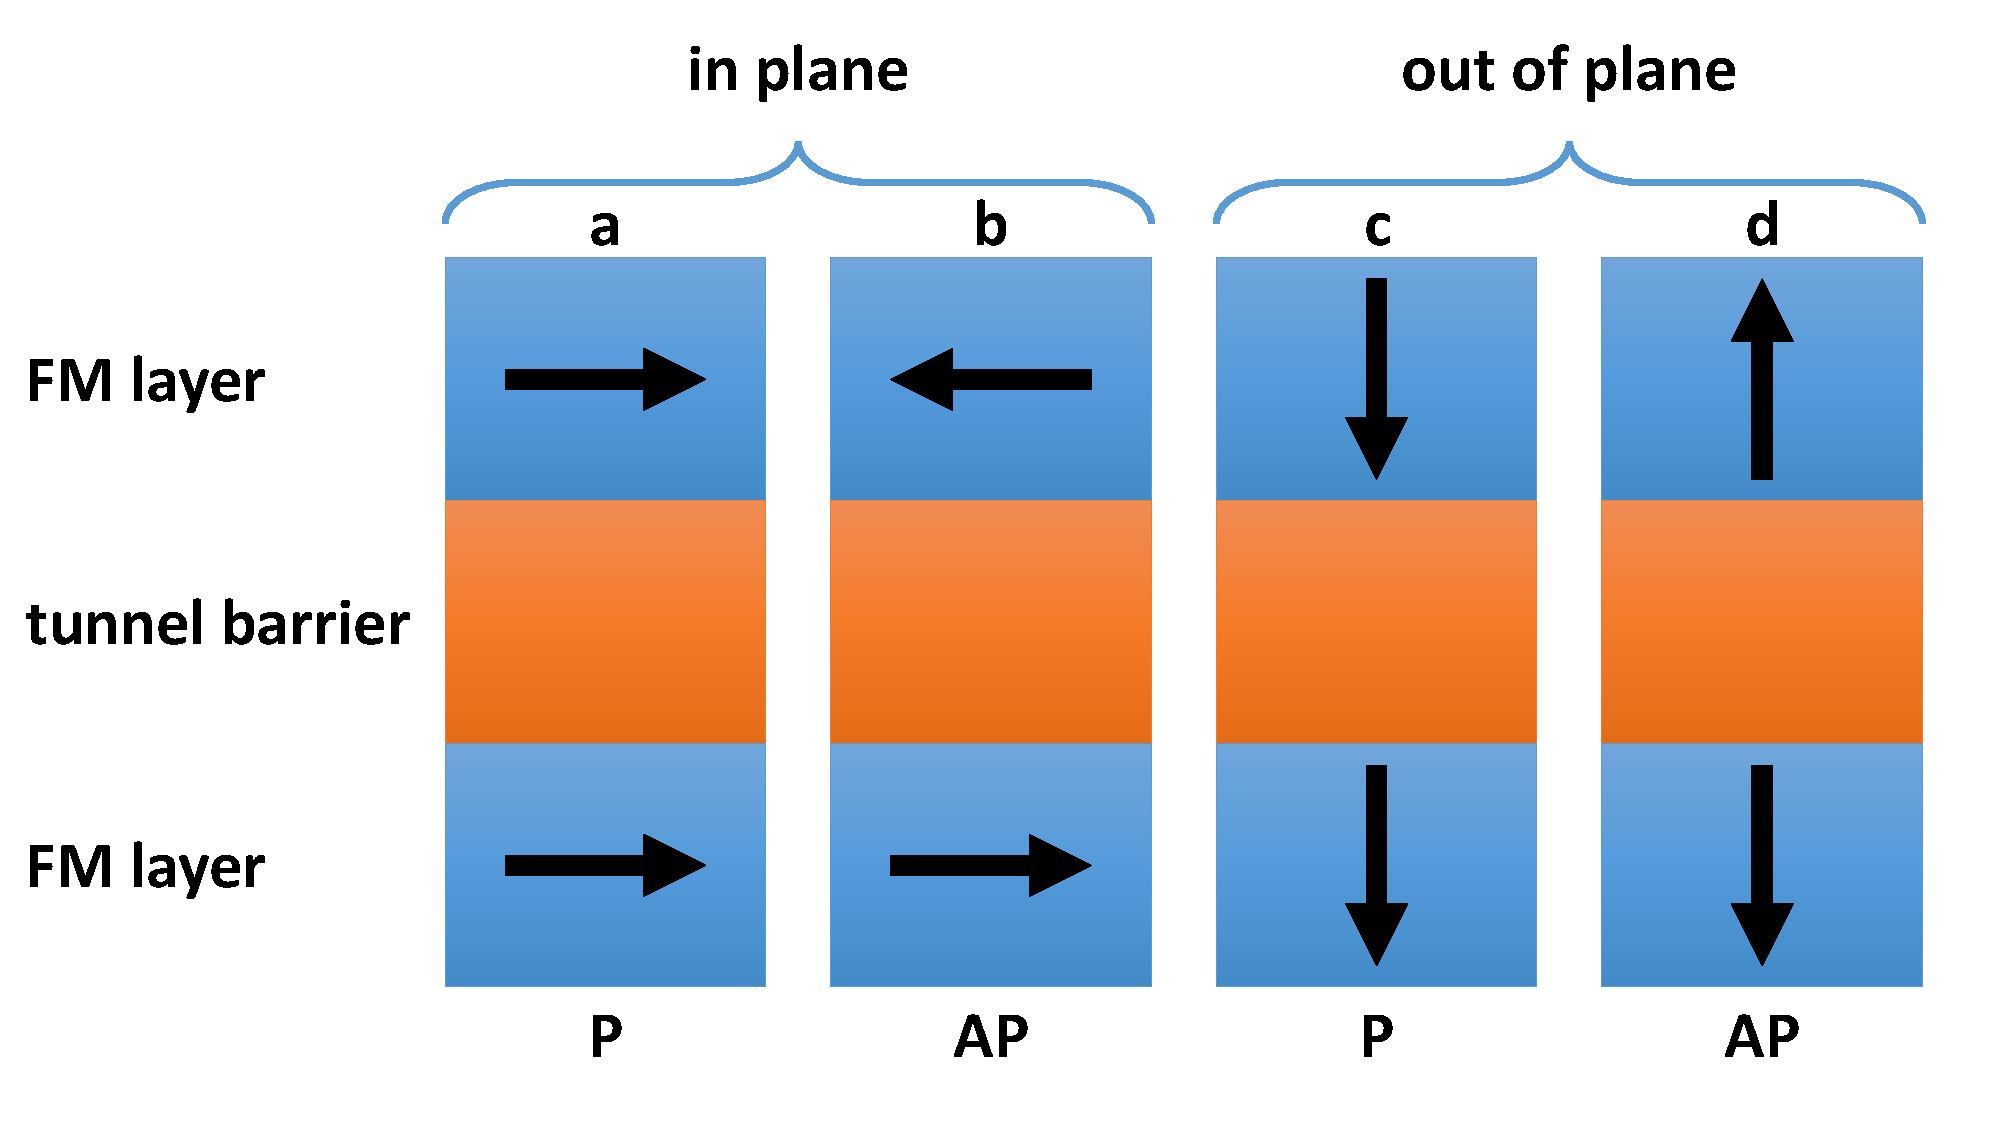
\includegraphics[width=0.75\paperwidth, page=1]{img/03/TMR_sch.pdf}
        \caption{Schematic of MTJ with IP anisotropy in P (a) and AP (b) state, and with PMA P (c) and AP (d) state. Arrows denote magnetisation vector of FM layers.}
        \label{PrinciplesMTJSchematic}
    \end{figure} 

\section{Tunnel magnetoresistance effect} \label{sec:PrinciplesTMR}

    The TMR effect is observed when FM layers separated by tunnel barrier exhibit different density of states $D$ in the $3d$ band (which also takes part in the tunneling process) at Fermi energy $E_F$ for electrons with spin oriented up ($D_\uparrow$) and down ($D_\downarrow$) (Fig. \ref{PrinciplesDOS}). Such materials are for example $Fe$, $Ni$, $Co$ or some alloys, like $CoFeB$ \cite{stobiecki2012urzadzenia}.
    
    \begin{figure}[H]
        \centering
        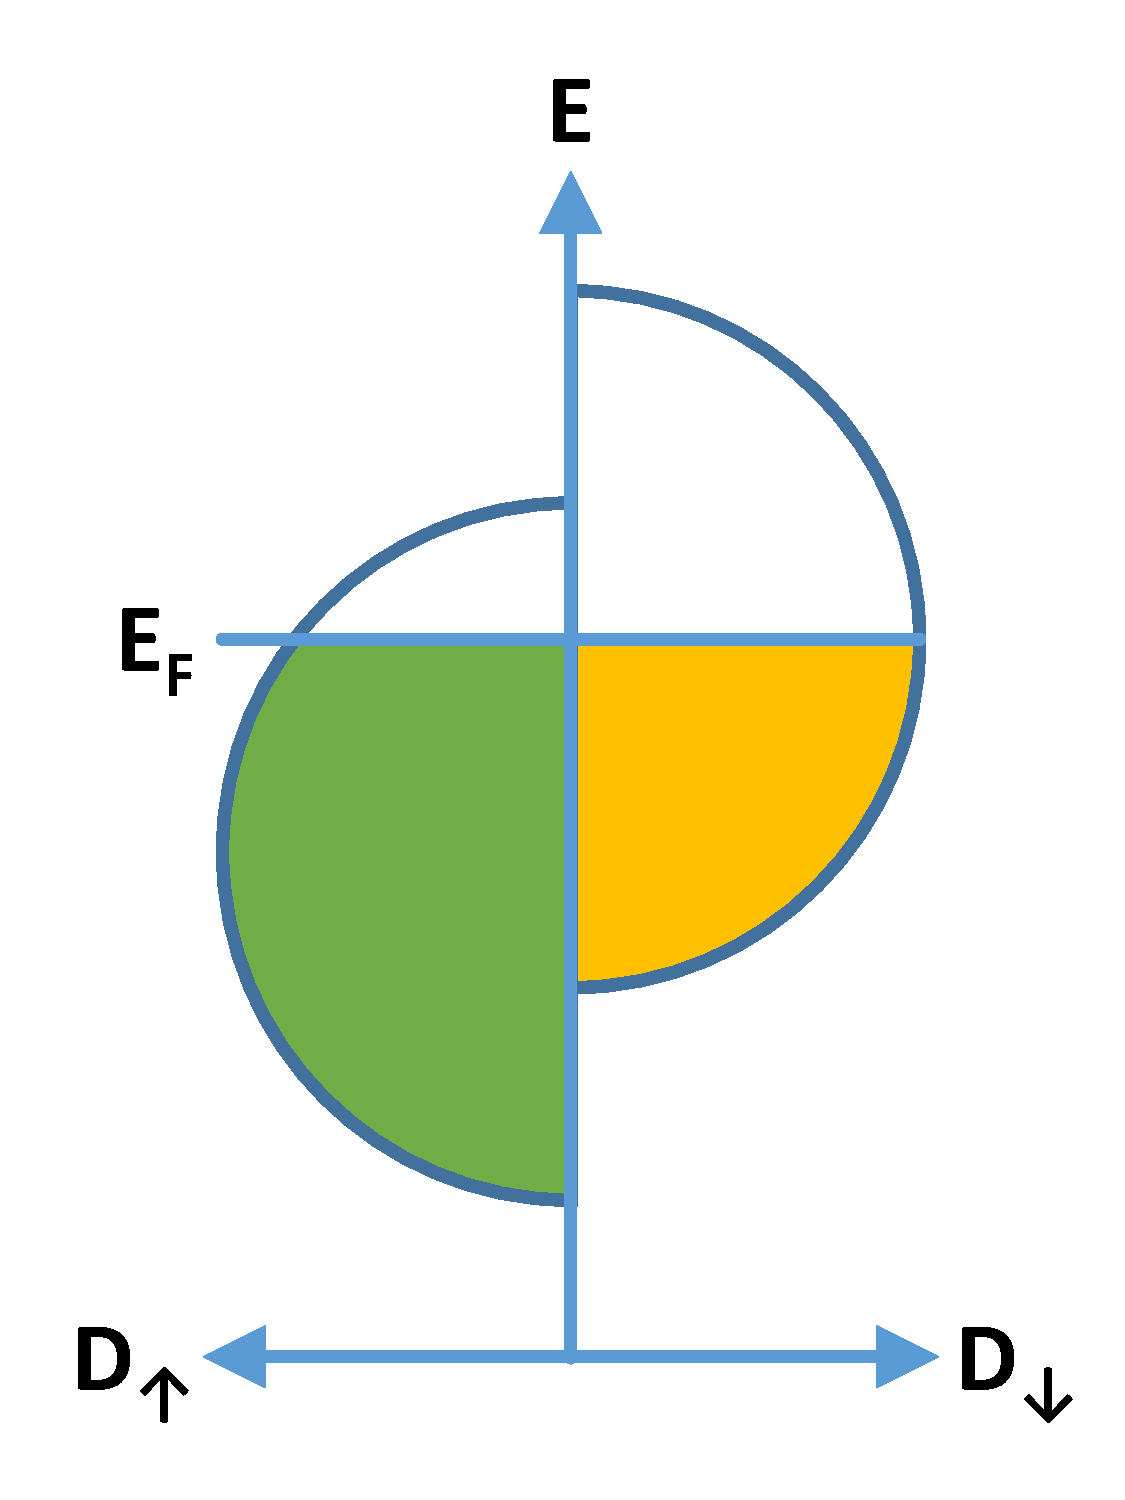
\includegraphics[width=0.20\paperwidth, page=1]{img/03/DOS_diagram.pdf}
        \caption{Schematic diagram of density of states in $3d$ band in $Fe$. Fermi energy is denoted.}
        \label{PrinciplesDOS}
    \end{figure} 
    
    Assuming that electrons are not changing their spin direction during tunnelling through barrier (which may be true only for sufficiently thin barriers; also electron flow is not fully spin-polarised) and must tunnel to sub-band with matching spin, the TMR effect can be explained in a simplified way presented below. 
    
    In the P state (Fig. \ref{PrinciplesTMRExplanation} a) there is relatively large amount of electrons with spin $\downarrow$ at $E_F$ available in the FM1 layer, and also in the FM2 layer there is plenty of space for the electrons at $E_F$ with spin $\downarrow$ - that results in a significant current flow of electrons with that spin. For electrons with spin $\uparrow$ - the amount in the FM1 layer at $E_F$ is small, and also available space in the FM2 layer is small, so the current of electrons with spin $\uparrow$ is small. Overall current is significant due to tunnelling of electrons with spin $\downarrow$, resulting in low resistance ($R_{P}$).
    
    In the AP state (Fig. \ref{PrinciplesTMRExplanation} b), as previously, the amount of electrons with spin $\downarrow$ available in the FM1 layer is high, but, due to opposite magnetisation of the FM2 layer, available space in the FM2 layer for those electrons is small, resulting in small current. Considering electrons with spin $\uparrow$ - there is plenty of space in the FM2 layer, but only limited amount in the FM1 layer - also resulting in small current flow. The overall current is small, so the resistance is large ($R_{AP}$) \cite{yuasa2007giant}. 
    
    The $TMR$ effect can be quantified as follows:
    
    \begin{equation} \label{eq:TMRdef}
		TMR = \frac{R_{AP}-R_{P}}{R_{P}}
	\end{equation}
According to the simple \citeauthor{julliere1975tunneling}'s model \cite{julliere1975tunneling} $TMR$ can also be expressed as a function of spin-polarisation of FM layers ($P_{FMx}$), which is the fraction of electrons that are becoming spin-polarized in each FM layer:
    
    \begin{equation} \label{eq:TMRpolarization}
		TMR = \frac{2\cdot P_{FM1}\cdot P_{FM2}}{1-P_{FM1}\cdot P_{FM2}},
	\end{equation}
however the nature of the phenomena is in reality much more complicated, and other factors are influencing the actual $TMR$, like for example spin filter effect in a tunnel barrier, the quality of FM / tunnel barrier interface or trapping states in tunnel barrier \cite{teixeira2011resonant}.

    \begin{figure}[H]
        \centering
        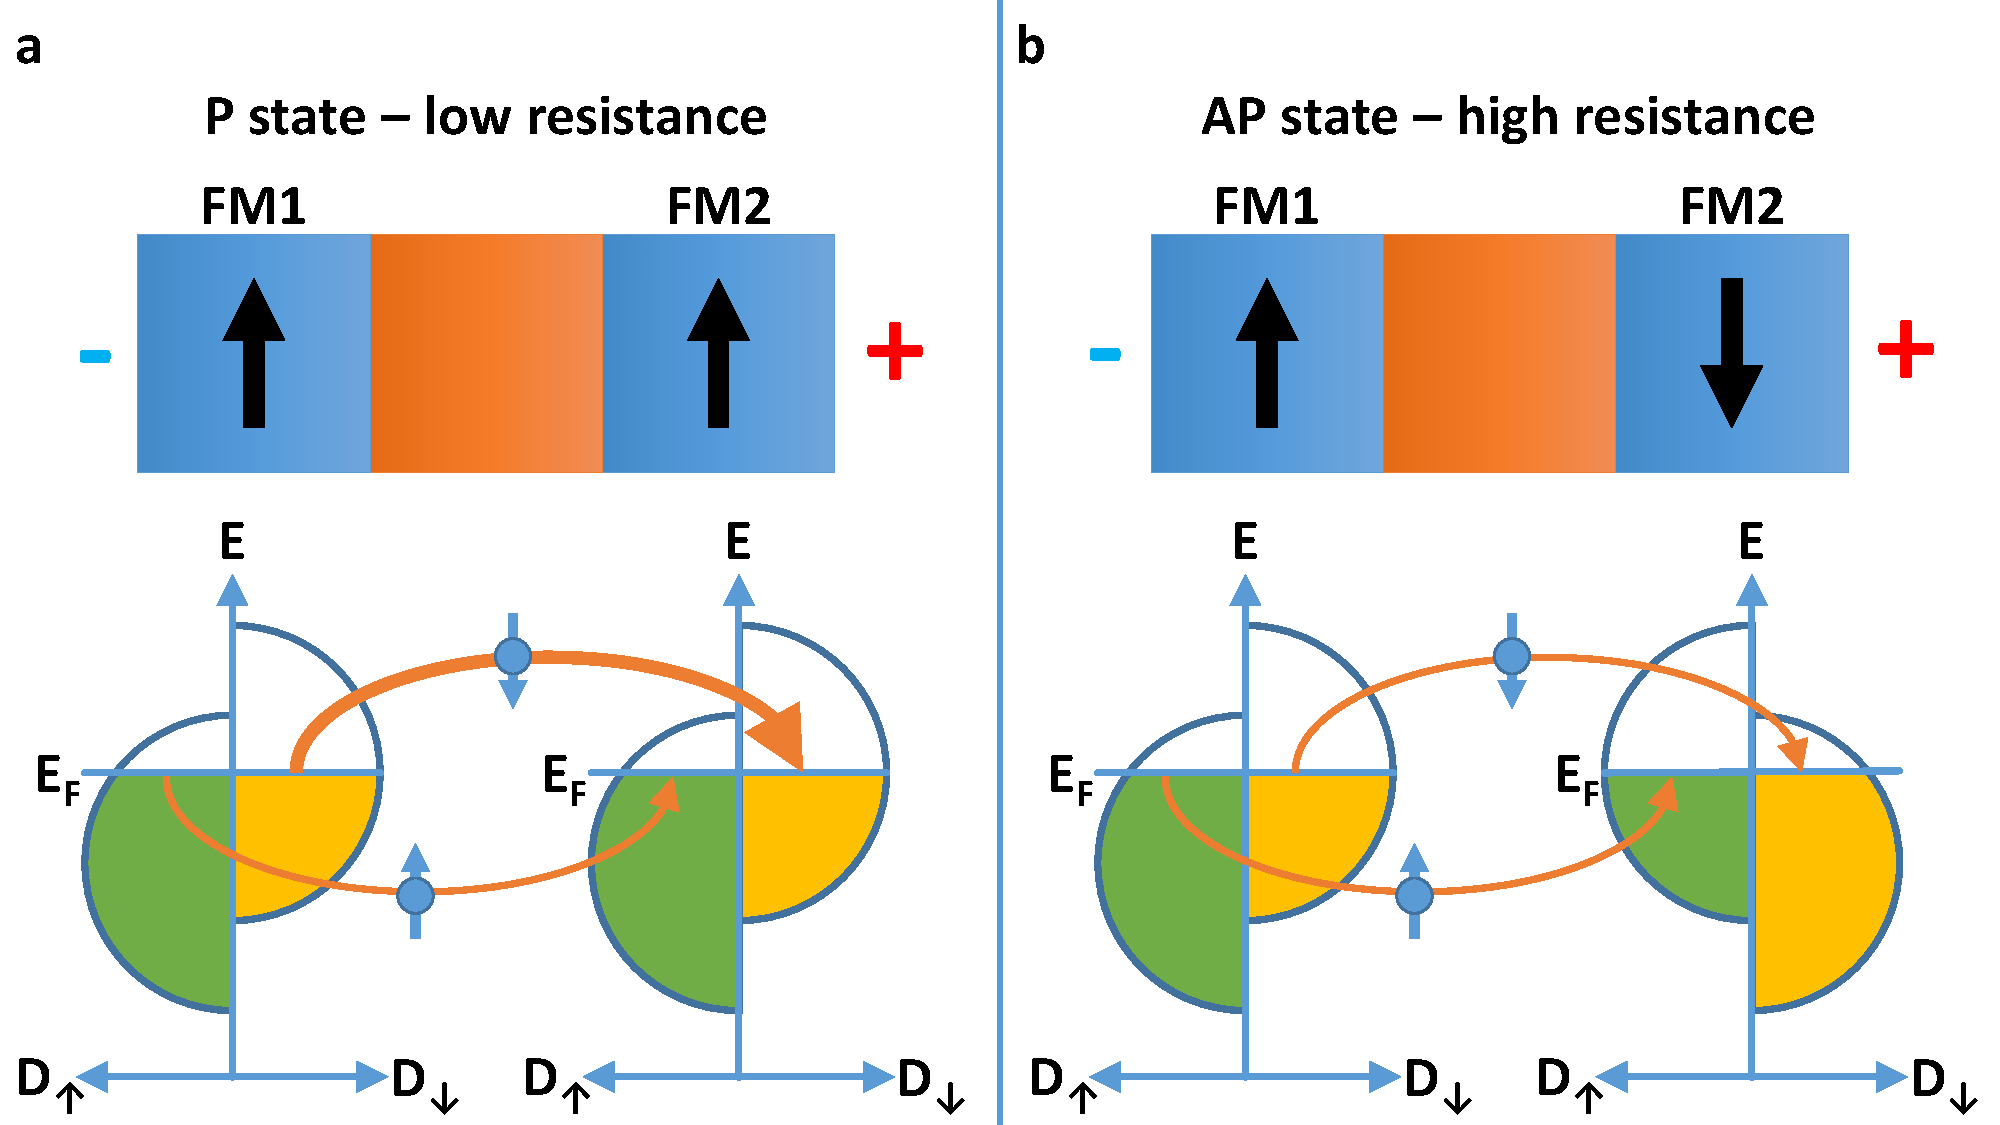
\includegraphics[width=0.75\paperwidth, page=1]{img/03/TMR_explanation.pdf}
        \caption{Schematic explanation of origin of TMR effect in MTJs. The thickness of orange arrows are proportional to current densities.}
        \label{PrinciplesTMRExplanation}
    \end{figure}	
	
	Also when considering layers having magnetization vectors at any relative angle $\theta$ (not only \SI{0}{\degree} for P and \SI{180}{\degree} for AP states), phenomenologically, the resistance of the MTJ can be expressed as the following function \cite{rijks1994interplay}:
	
	\begin{equation} \label{eq:Rangular}
		R(\theta) = R_P + \frac{R_{AP} - R_P}{2}(1-cos\theta).
	\end{equation}

\section{Defining reference layer by pinning} \label{sec:PrinciplesAdditionalPinning}

    To produce a working MRAM storage element it is important to define one FM layer as a storage layer (of which magnetisation direction is to be changed while writing, so called free layer - FL) and the second as a fixed layer (or reference layer - RL), of which magnetisation direction should be hard to change. Without that one can observe pseudo spin valve (PSV) behaviour presented in Fig. \ref{PrinciplesPSV}. As the bottom FM layer (FM2) is nearly as easy to magnetize, as the top one (FM1), hysteresis loops are very narrow. This justifies the need of pining one of the layers and defining the RL.
    
    \begin{figure}[H]
        \centering
        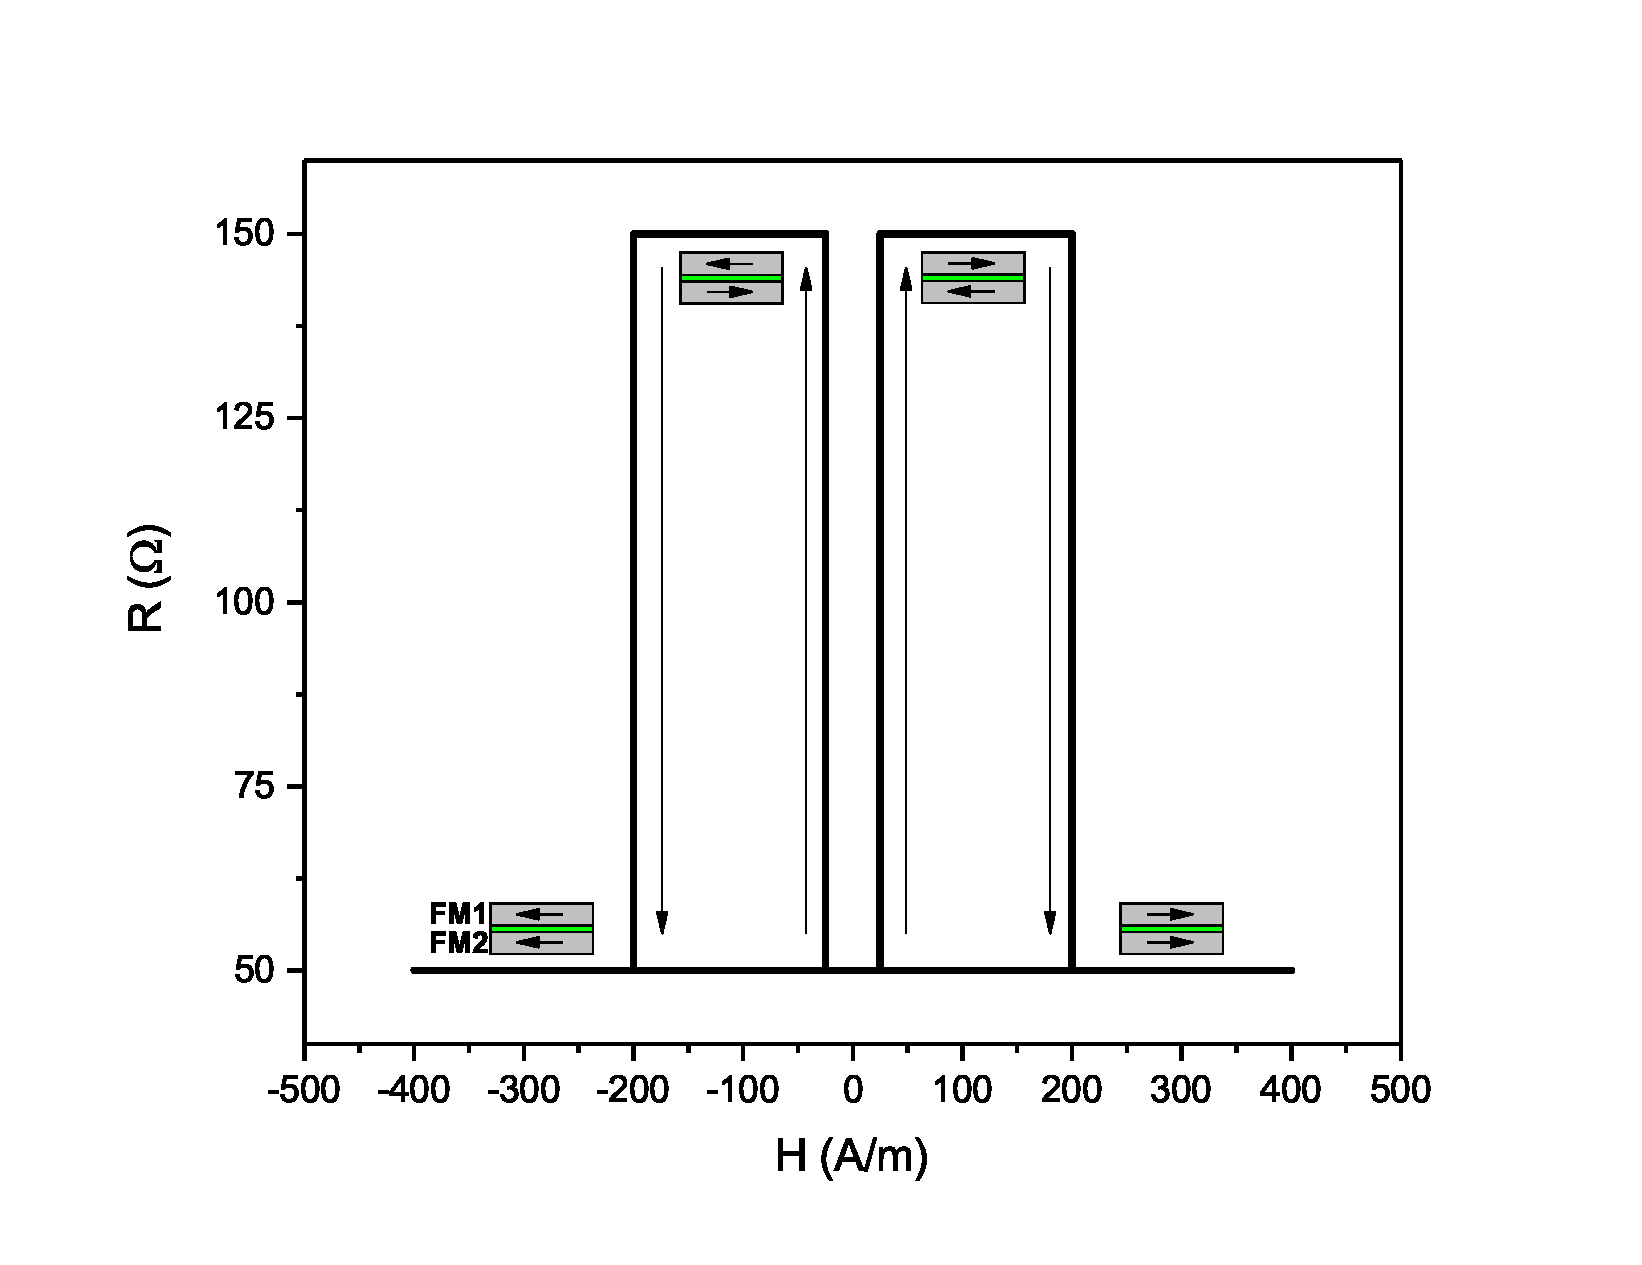
\includegraphics[width=0.7\paperwidth]{img/03/MTJ_characteristics_PSV.eps}
        \caption{PSV behaviour in external magnetic field $H$. Magnetization directions of both FM layers presented in stable states.}
        \label{PrinciplesPSV}
    \end{figure}    
    
    Different coupling mechanisms between thin FM layers were discovered, depending on the type of the spacer. The Ruderman–Kittel–Kasuya–Yosida (RKKY) \cite{yosida1957magnetic} coupling is measured between FM layers separated by a non-magnetic (NM) metallic layer (Fig. \ref{PrinciplesSAF} a). Depending on NM layer thickness, the coupling can be both ferromagnetic and anti-ferromagnetic, resulting in magnetsation vectors with the same, and opposite direction, respectively \cite{stobiecki2012urzadzenia}. 
    
    By intentionally coupling two FM layers a synthetic anti-ferromagnet is created. One of the FM layers can be used as RL in MTJ (Fig. \ref{PrinciplesSAF} b) \cite{bandiera2010comparison, zhu1999spin}, as well as additional layers may be coupled to the SAF for the purpose \cite{wang2015tunnel}.
    
    When anisotropy is not defined mainly by dimensions (size and thickness), a natural AF (e.g. $IrMn$) is used to induce unidirectional anisotropy in one of the SAF layers (Fig. \ref{PrinciplesSAF} c).
    
    The second type of coupling, namely an interlayer exchange coupling (IEC) exists between FM layers separated by an insulator layer (e.g. $MgO$ tunnel barrier) \cite{katayama2006interlayer,jiancheng2015effect}. This coupling causes the shift of the hysteresis loop (Sec. \ref{sec:PrinciplesRHmeas}, Eq. \ref{eq:TMRsato}). In practice, it is vital to reduce the influence, because the lower the shift, the more symmetrical the switching currents. Reduction of the IEC can be done by using careful design of SAF and SAF-like structures for the top FM layer.
    
    \begin{figure}[H]
        \centering
        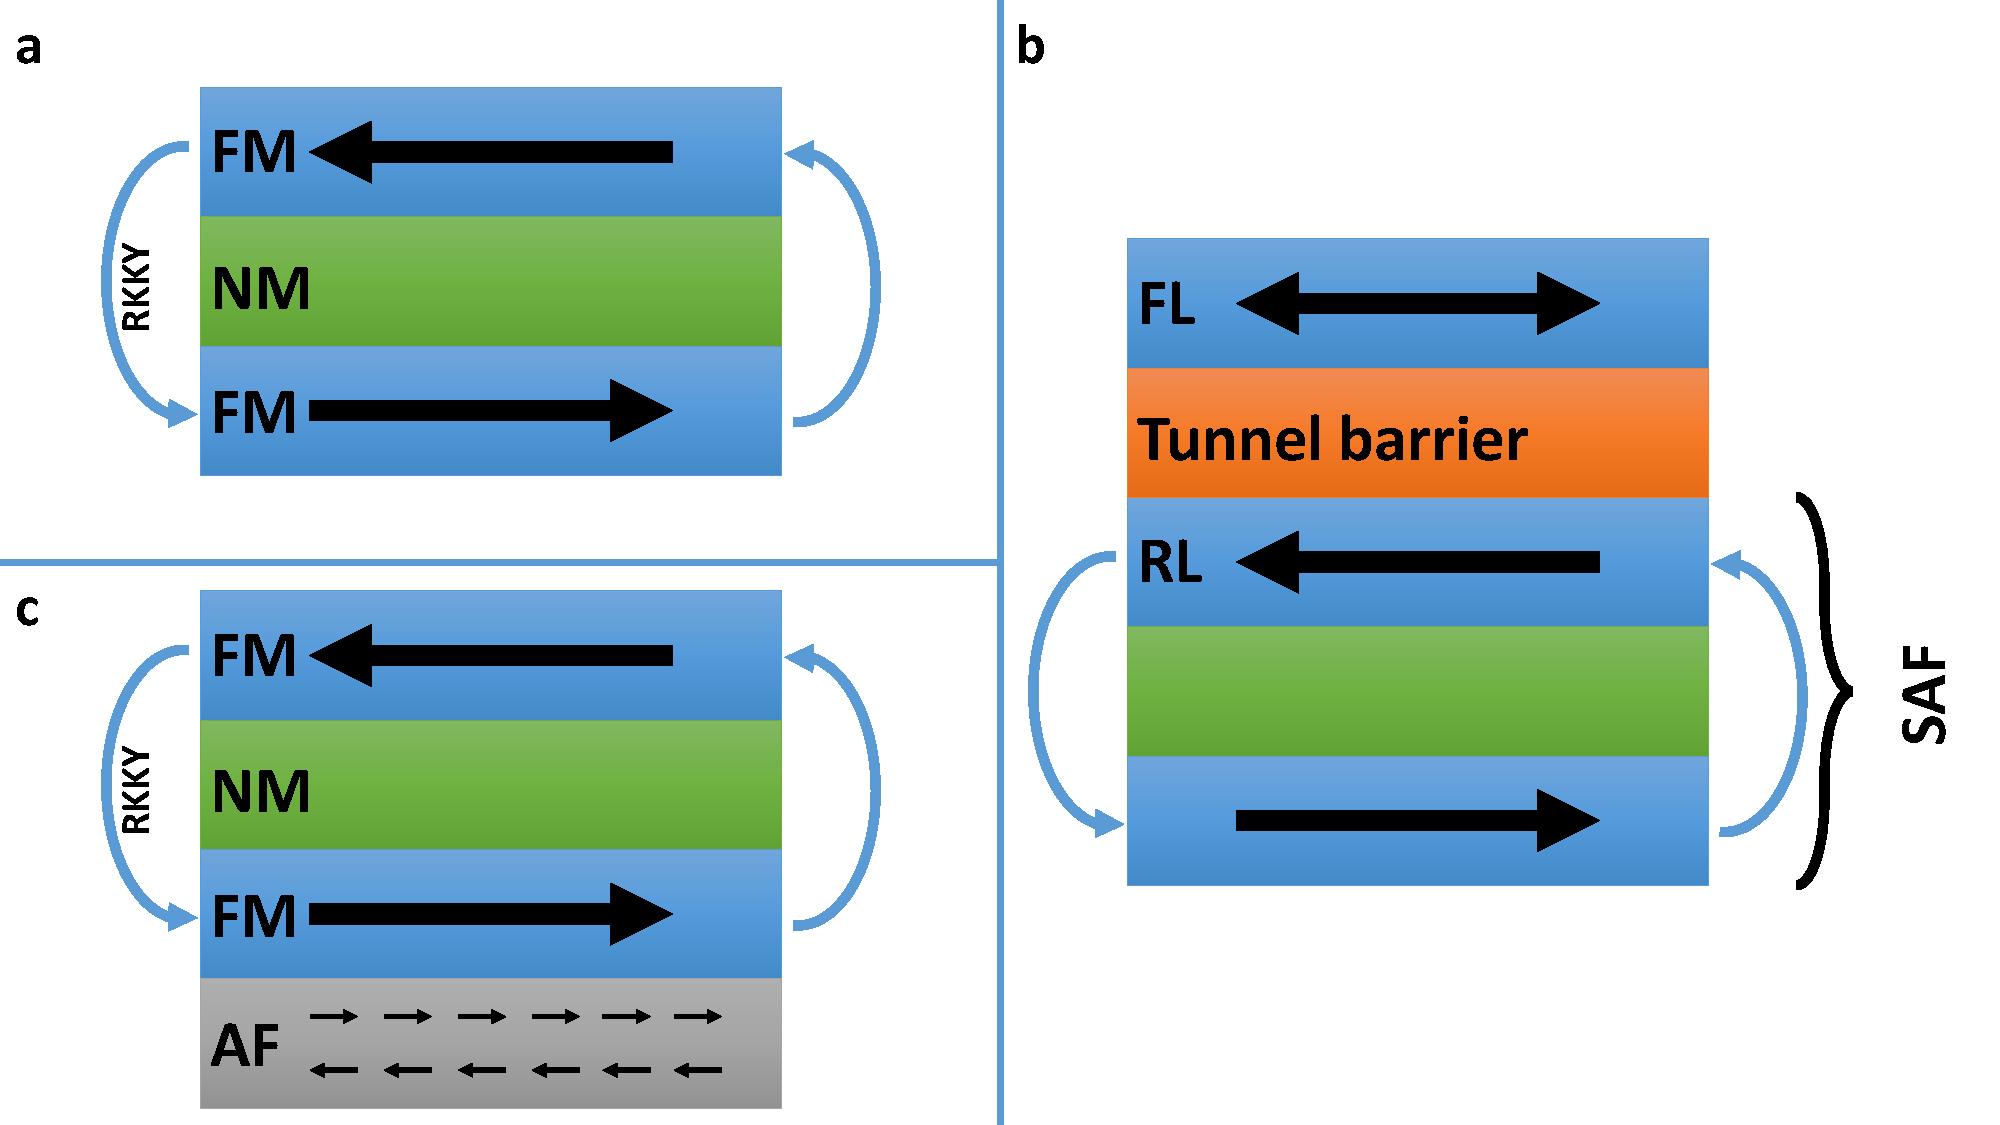
\includegraphics[width=0.75\paperwidth, page=1]{img/03/Pinning.pdf}
        \caption{a) RKKY anti-ferromagnetic coupling between two FM layers separated by NM metallic spacer. b) Schematic of MTJ junction with RL pinned using SAF structure. c) Additional AF used to induce anisotropy in the bottom FM layer.}
        \label{PrinciplesSAF}
    \end{figure} 
    
\section{Behaviour of the MTJ with pinned layer}
\label{sec:PrinciplesRHmeas}   
    The storage element can be primarily characterised using $R(H)$ measurement, i.e.\ resistance ($R$) versus external magnetic field ($H$) applied parallel to the anisotropy of the sample. This measurement allows to determine TMR of the examined MTJ, and therefore it is called a TMR measurement. Theoretical characteristics are presented in Fig. \ref{PrinciplesMTJtmr} together with illustrated orientation of RL and FL in characteristic regions.
    
    When applying low magnetic field only FL is changing its magnetisation and, depending on the orientation of RL, two different minor hysteresis loops (symmetrical to each other) can be observed (Fig. \ref{PrinciplesMTJtmr} a, b). Usually each minor loop tends not to be symmetrical around zero field, due to coupling between FL and RL. Applying sufficiently strong fields results in switching of RL, and a major hysteresis loop is observed (Fig. \ref{PrinciplesMTJtmr} c), in contrast to PSV, when smaller magnetic field caused such behaviour (Fig. \ref{PrinciplesPSV}).
    
    By repeating $R(H)$ measurements (Fig. \ref{PrinciplesMTJtmr} a or b) multiple times in the same conditions, and by changing the magnetic field slow enough, a distribution of magnetic field for switching from P to AP and vice versa can be obtained. Using the formula (Eq. \ref{eq:TMRsato}) presented by \citeauthor{sato2012cofeb} to fit the experimental data, a thermal stability ($\Delta$) can be obtained as well as other important parameters \cite{sato2012cofeb}. The formula was corrected from the originally presented version, by inserting absolute value.
    
    \begin{figure}[H]
        \centering
        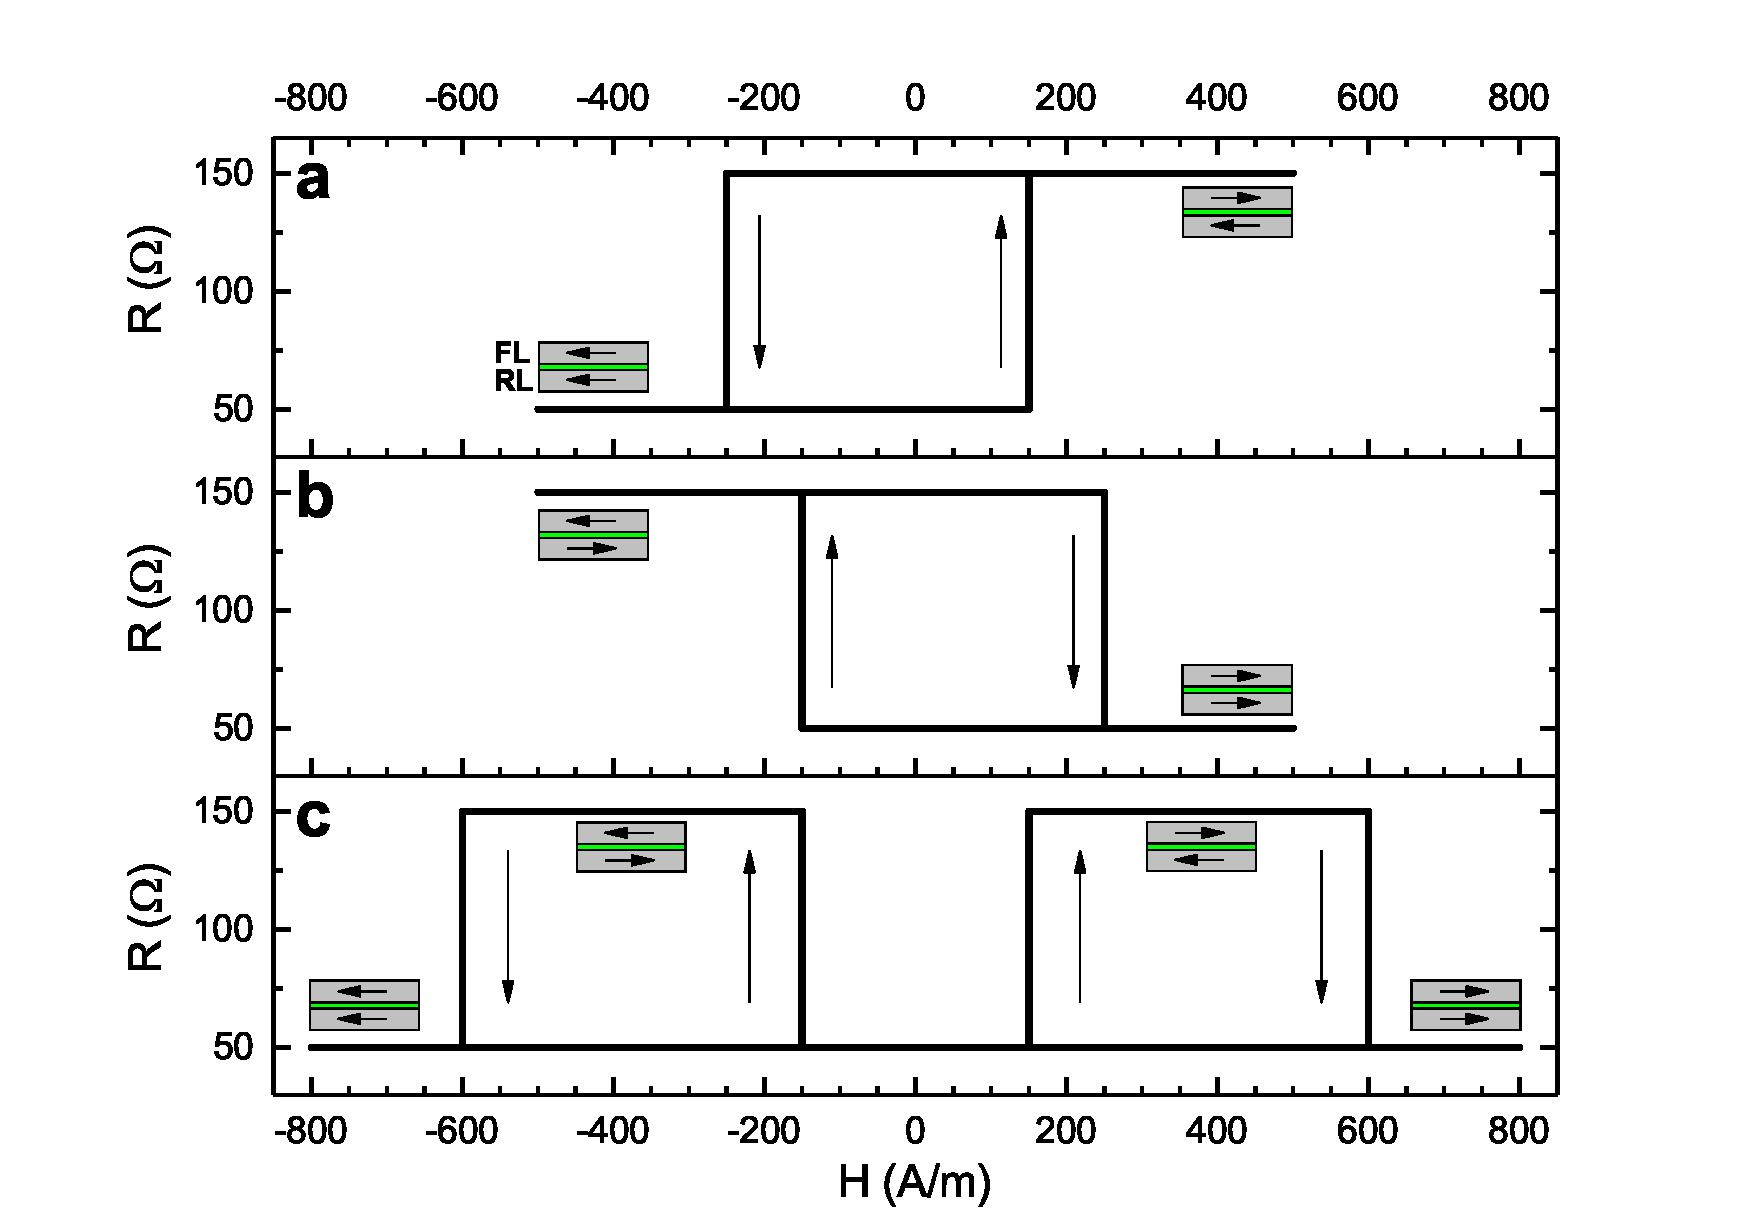
\includegraphics[width=0.75\paperwidth]{img/03/MTJ_characteristics.eps}
        \caption{Theoretically predicted characteristics of MTJ resistance versus external magnetic field applied in a direction parallel to the anisotropy of the MTJ (with orientation of FL (upper) and RL (lower) in characteristic regions) when: a) and b) only FL is switching in lower fields, c) RL is switching in higher fields.}
        \label{PrinciplesMTJtmr}
    \end{figure}
    
    \begin{equation} \label{eq:TMRsato}
		P(\tau) = 1 - exp\left [ -\frac{\tau}{\tau_0}exp\left \{ -\Delta\left ( 1-\frac{|H-H_s|}{H_k^{eff}} \right ) \right \} \right ]
	\end{equation}
In Eq. \ref{eq:TMRsato} $\tau$ denotes the magnetic field step duration (in the study \SI{1}{\second}), $\tau_0$ the inverse of attempt frequency (in the thesis assumed to be \SI{1}{\nano\second}), $\Delta$ the thermal stability, $H$ the external magnetic field, $H_s$ shift field of the TMR loops (i.e. the field between zero and the center of $R(H)$ hysteresis loop) and $H_k^{eff}$ denotes the effective magnetic anisotropy field. The thermal stability is expressed as:

	\begin{equation} \label{eq:TMRsatoDelta}
		\Delta = \frac{E}{k_bT},
	\end{equation}
where $E$ denotes the energy barrier between P and AP states, $k_b$ the Boltzmann constant and $T$ denotes the absolute temperature (in the experiment \SI{300}{\kelvin}). For practical applications thermal stability should be $\Delta \geq 60$ \cite{apalkov2010comparison}.

\section{Spin transfer torque (STT) and current induced magnetisation switching (CIMS) effects} \label{sec:PrinciplesCIMS}

    In order to switch the magnetisation of the storage layer (FL) one can apply external magnetic field or use the spin transfer torque phenomenon \cite{bhatti2017spintronics}. When using external magnetic field to switch the storage element, additional current lines need to be present, to generate Oersted field. This require additional area inside the memory chip and is not energy-efficient \cite{kent2015new,fujisaki2013review}. On the other hand, using the STT effect does not require current lines for write operation, and uses less energy. To understand the STT phenomenon, two cases need to be analysed: switching from AP to P state, and vice versa. The explanation presented below uses a simplified model, as the nature of the phenomenon is very complex.
    
    When the MTJ is initially in the AP state (Fig. \ref{PrinciplesSTTsch} a), in order to switch the magnetization of the FL electrons must flow upwards (from RL to FL). Electrons are spin-polarised by RL and a considerable amount of them does not change its spin during tunnelling. As they enter FL, magnetization of which is oriented in the opposite way, they need to change their spin, and, therefore, angular momentum. This momentum change induces torque (called spin transfer torque), that rotates magnetization of the FL. If the amount of electrons is big enough, the STT can cause the magnetization to flip to the opposite stable position (P) - the process is called current induced magnetisation switching (CIMS). A current which induces CIMS is called the critical current.
    
    When the MTJ is in P state (Fig. \ref{PrinciplesSTTsch} b) to switch the magnetization of the FL, electrons must flow from FL to RL (downwards). Electrons are spin-polarised by FL and some of them reverse their spin during tunnelling. As RL is pinned, it is more energy-efficient to return to the FL, rather then tunnelling to RL. These electrons now have spin opposite to the magnetisation of FL, so they are generating STT. With sufficient amount of these electrons CIMS effect takes place to change the MTJ state to AP.
    
%\subsection{CIMS measurement result prediction}
\label{sec:PrinciplesCIMSmeas}   
    A CIMS, as discussed above, can be induced by applying a voltage across the MTJ. When the voltage induces sufficient current the CIMS occurs, what is presented in Fig. \ref{PrinciplesMTJcims}. Such measurement, conducted in constant external magnetic field $H$, is called a CIMS measurement. It is important to notice, that when the resistance changes with constant voltage applied, the current also increases or decreases abruptly (Fig. \ref{PrinciplesMTJcims} b). Additionally, by performing series of such measurements in different external magnetic fields and marking voltages of CIMS and the field, a stability diagram can be obtained \cite{skowronski2017understanding}. The diagram (Fig. \ref{PrinciplesEye} shows regions (in voltage-field coordinates) where only P, AP, or both of the states are possible.
    
    \begin{figure}[H]
        \centering
        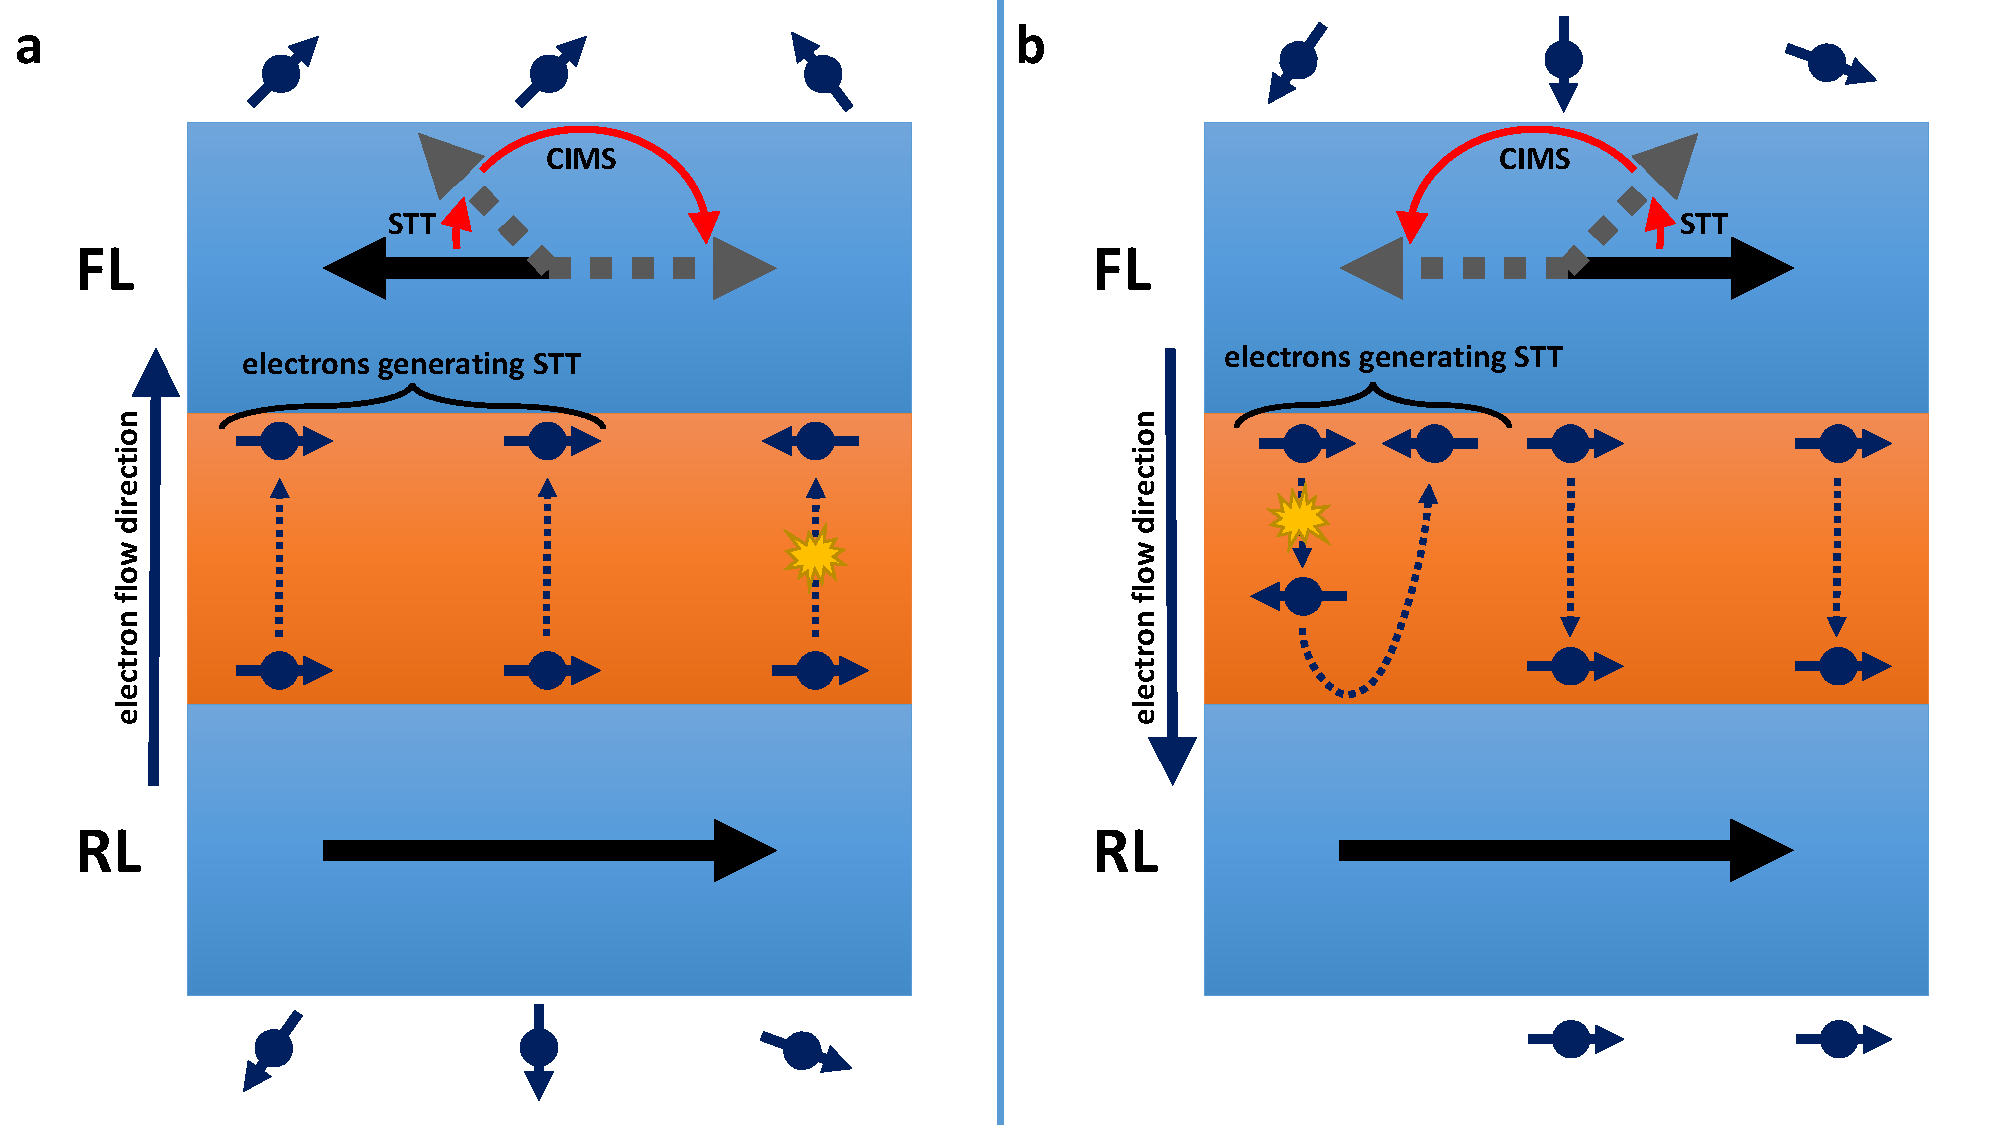
\includegraphics[width=0.75\paperwidth, page=1]{img/03/STT_sch.pdf}
        \caption{Schematic explanation of CIMS process for switching from AP to P (a) and from P to AP (b). For better illustration, IP anisotropy was presented.}
        \label{PrinciplesSTTsch}
    \end{figure}
    
    \begin{figure}[H]
        \centering
        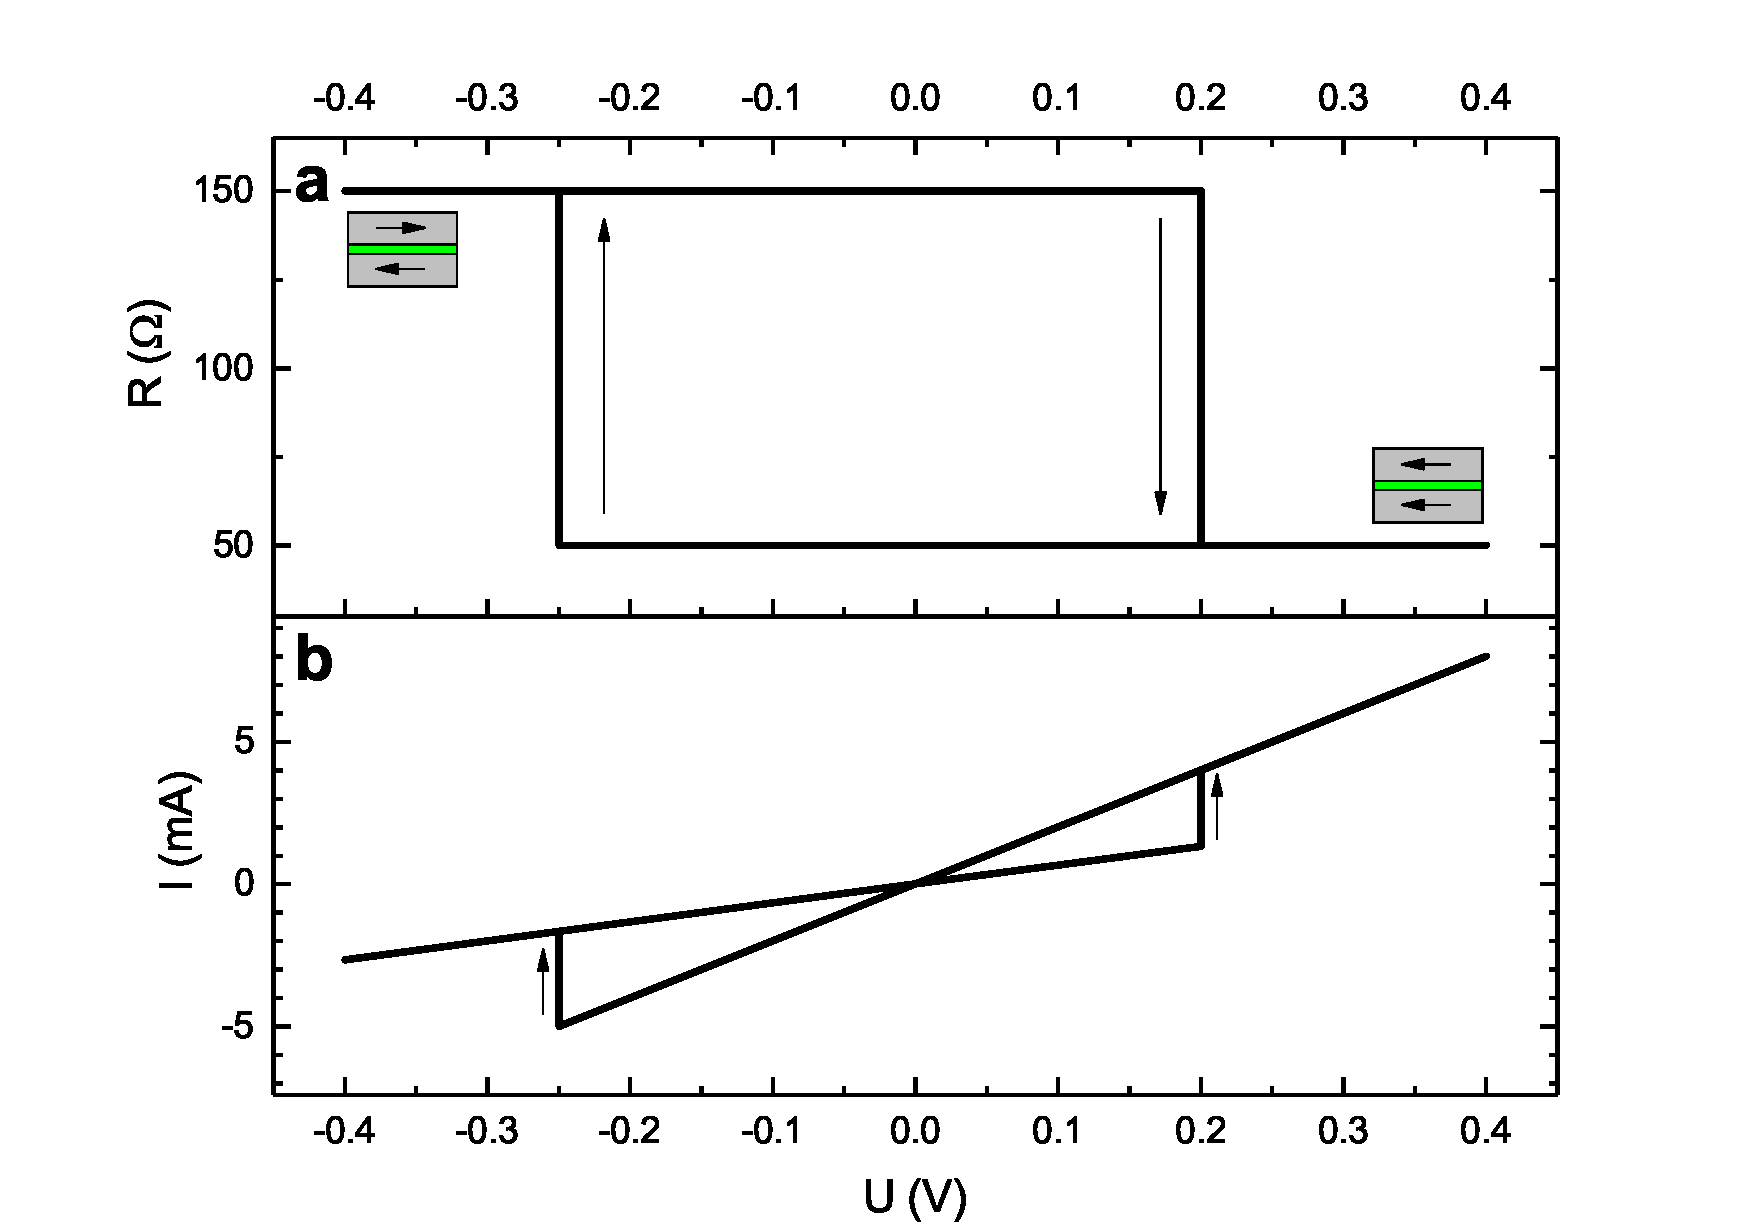
\includegraphics[width=0.75\paperwidth]{img/03/MTJ_characteristics_CIMS.eps}
        \caption{Theoretically predicted a) resistance and b) current versus voltage applied to an MTJ. A CIMS may be observed.}
        \label{PrinciplesMTJcims}
    \end{figure}
    
    \begin{figure}[H]
        \centering
        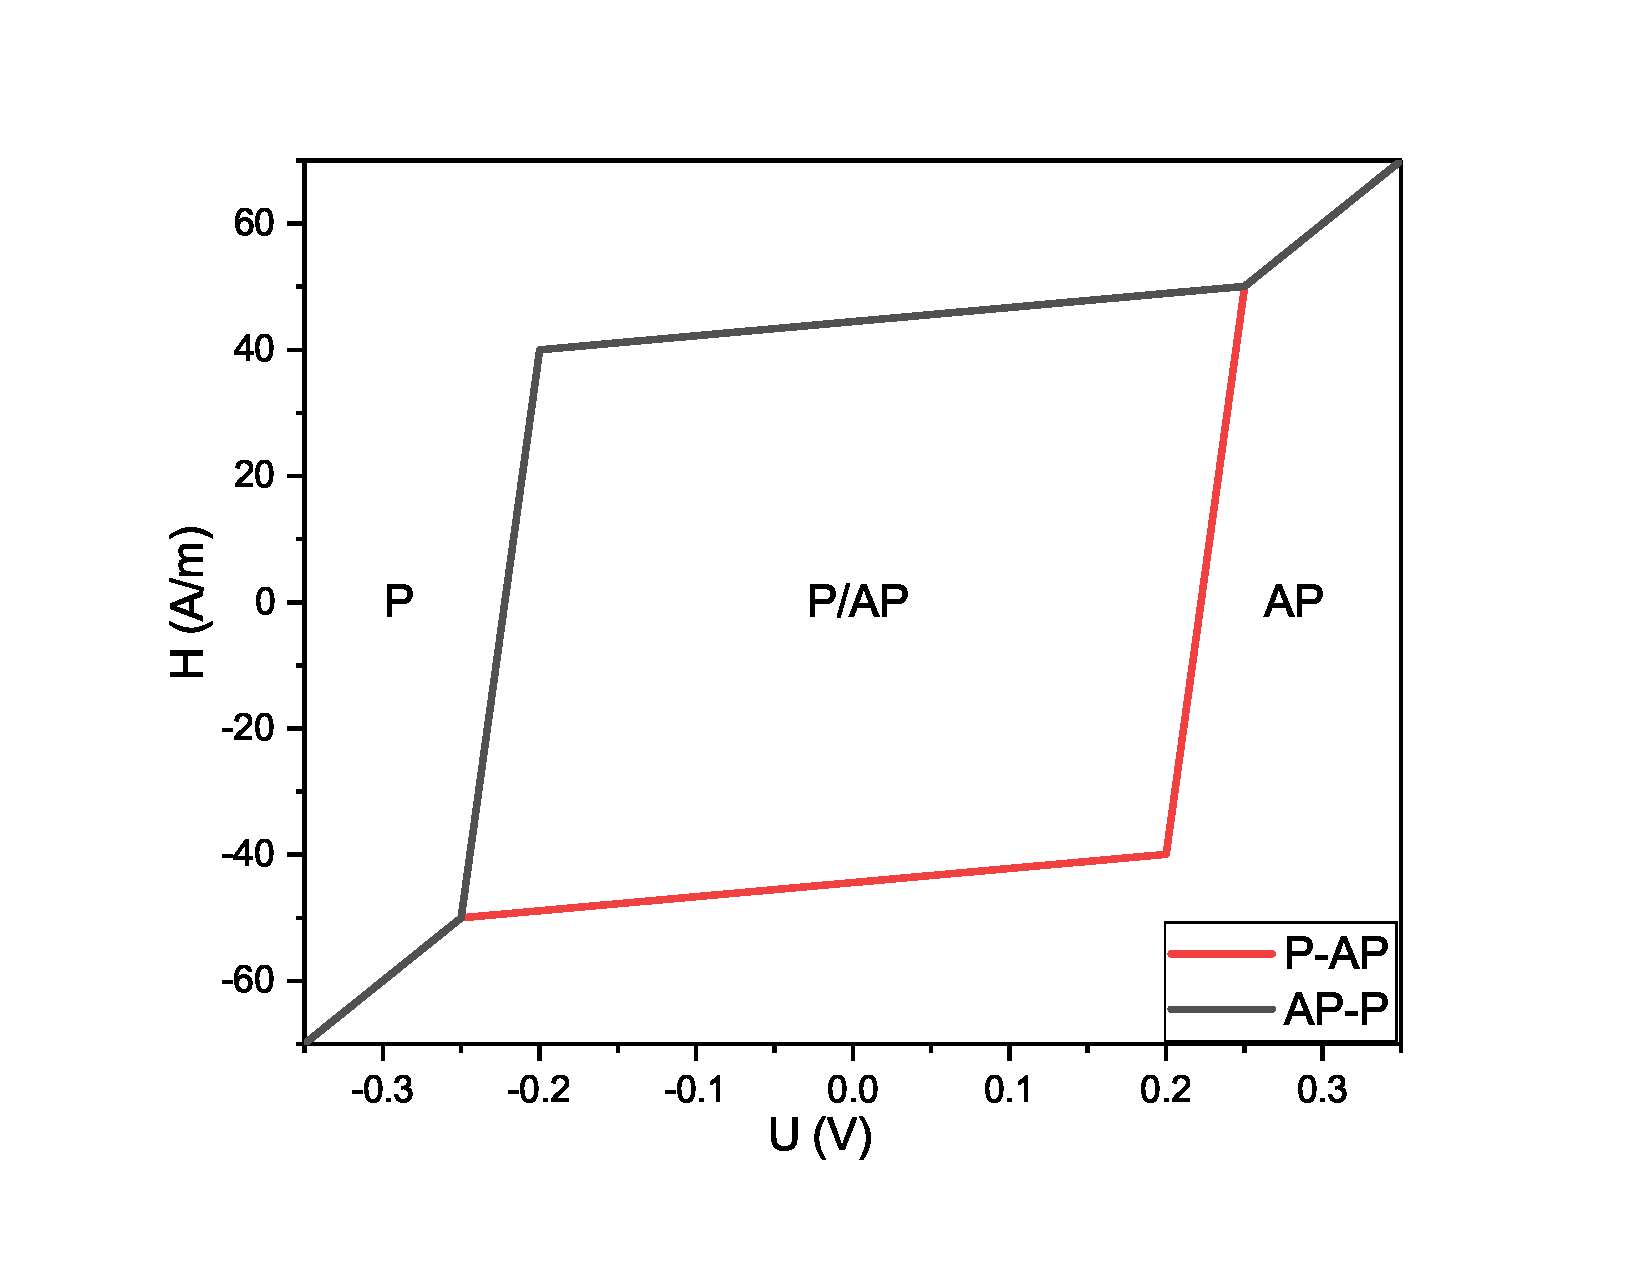
\includegraphics[width=0.75\paperwidth]{img/03/Eye_example.eps}
        \caption{Theoretically predicted stability diagram. Lines indicate switching from P to AP or vice versa. Regions are marked with possible states of an MTJ (P, P/AP, AP).}
        \label{PrinciplesEye}
    \end{figure}
    
\section{Perpendicular magnetic anisotropy} \label{sec:PrinciplesAdditionalPerpendicular}

    To understand the need of using PMA in MRAM storage elements, critical currents ($I_C$) need to be taken into account. With the use of the model presented by \citeauthor{mangin2006current}, critical currents for IP anisotropy and PMA can be approximated as follows \cite{mangin2006current}:
    
    \begin{equation} \label{eq:IcIP}
		I_C^{IP}\approx \frac{A\alpha M_SV}{g(\theta)p}(H+H_{dip}\varpm H_{K\parallel}\varpm \frac{M_S}{2})\mu_0
	\end{equation}
	
	\begin{equation} \label{eq:IcPMA}
		I_C^{PMA}\approx \frac{A\alpha M_SV}{g(\theta)p}(-H-H_{dip}\varpm H_{K\bot}\varmp M_S)\mu_0
	\end{equation}
In the above equations \ref{eq:IcIP} (for IP anisotropy) and \ref{eq:IcPMA} (for PMA) $M_S$, $V$ and $\alpha$ are the saturation magnetization, volume and Gilbert damping constant for FL, respectively, $\theta$ is the relative angle between magnetizations of FL and RL, and the $g$ factor depends on this angle, $p$ is the magnitude of the angular dependence, $A$ is a phenomenological factor dependent on transport model used, and it's unit is \si{\per\weber}. $H$ is the external magnetic field applied parallel to the easy axis of magnetization, $H_{dip}$ is the dipole field from the RL acting on the FL. $H_{K\parallel}$ and $H_{K\bot}$ are the uniaxial IP anisotropy or PMA fields, respectively. \SI[parse-numbers = false, number-math-rm = \ensuremath]{\theta = 180}{\degree} and operators in brackets are true for AP to P switching, and \SI[parse-numbers = false, number-math-rm = \ensuremath]{\theta = 0}{\degree} and operators without brackets are true for switching from P to AP.
    
    A potential advantage of PMA is that the critical currents for switching the magnetization (for small $H$ and $H_{dip}$, which are true for no external magnetic field and reduced IEC) are directly proportional to the anisotropy $H_{K\bot}$, and, hence, the stability of the bit. For the IP devices the current must overcome the additive factor $\frac{M_S}{2}$ that does not contribute to the stability of the bit against thermal fluctuations, but suppresses CIMS. Therefore, storage elements with PMA have lower write energies than the ones with IP anisotropy \cite{kishi2008lower,frankowski2015buffer}. The PMA can be obtained by using sufficiently thin layer of ferromagnetic material (Fig. \ref{PrinciplesPerpendicular} a) \cite{kisielewski2004wide}.
    
    As the effect described above takes place for thickness about \SI{1}{\nano\meter}, the volume of the layer after forming of the pillar is too small to observe an effect suitable for the application. In order to increase effective thickness, while maintaining out of plane anisotropy, a multilayer has to be deposited, with alternating FM and non-magnetic materials (such as $Pt$ or $Pd$) (Fig. \ref{PrinciplesPerpendicular} b) \cite{kim2017cofesib, park2008co}.
    
    \begin{figure}[H]
        \centering
        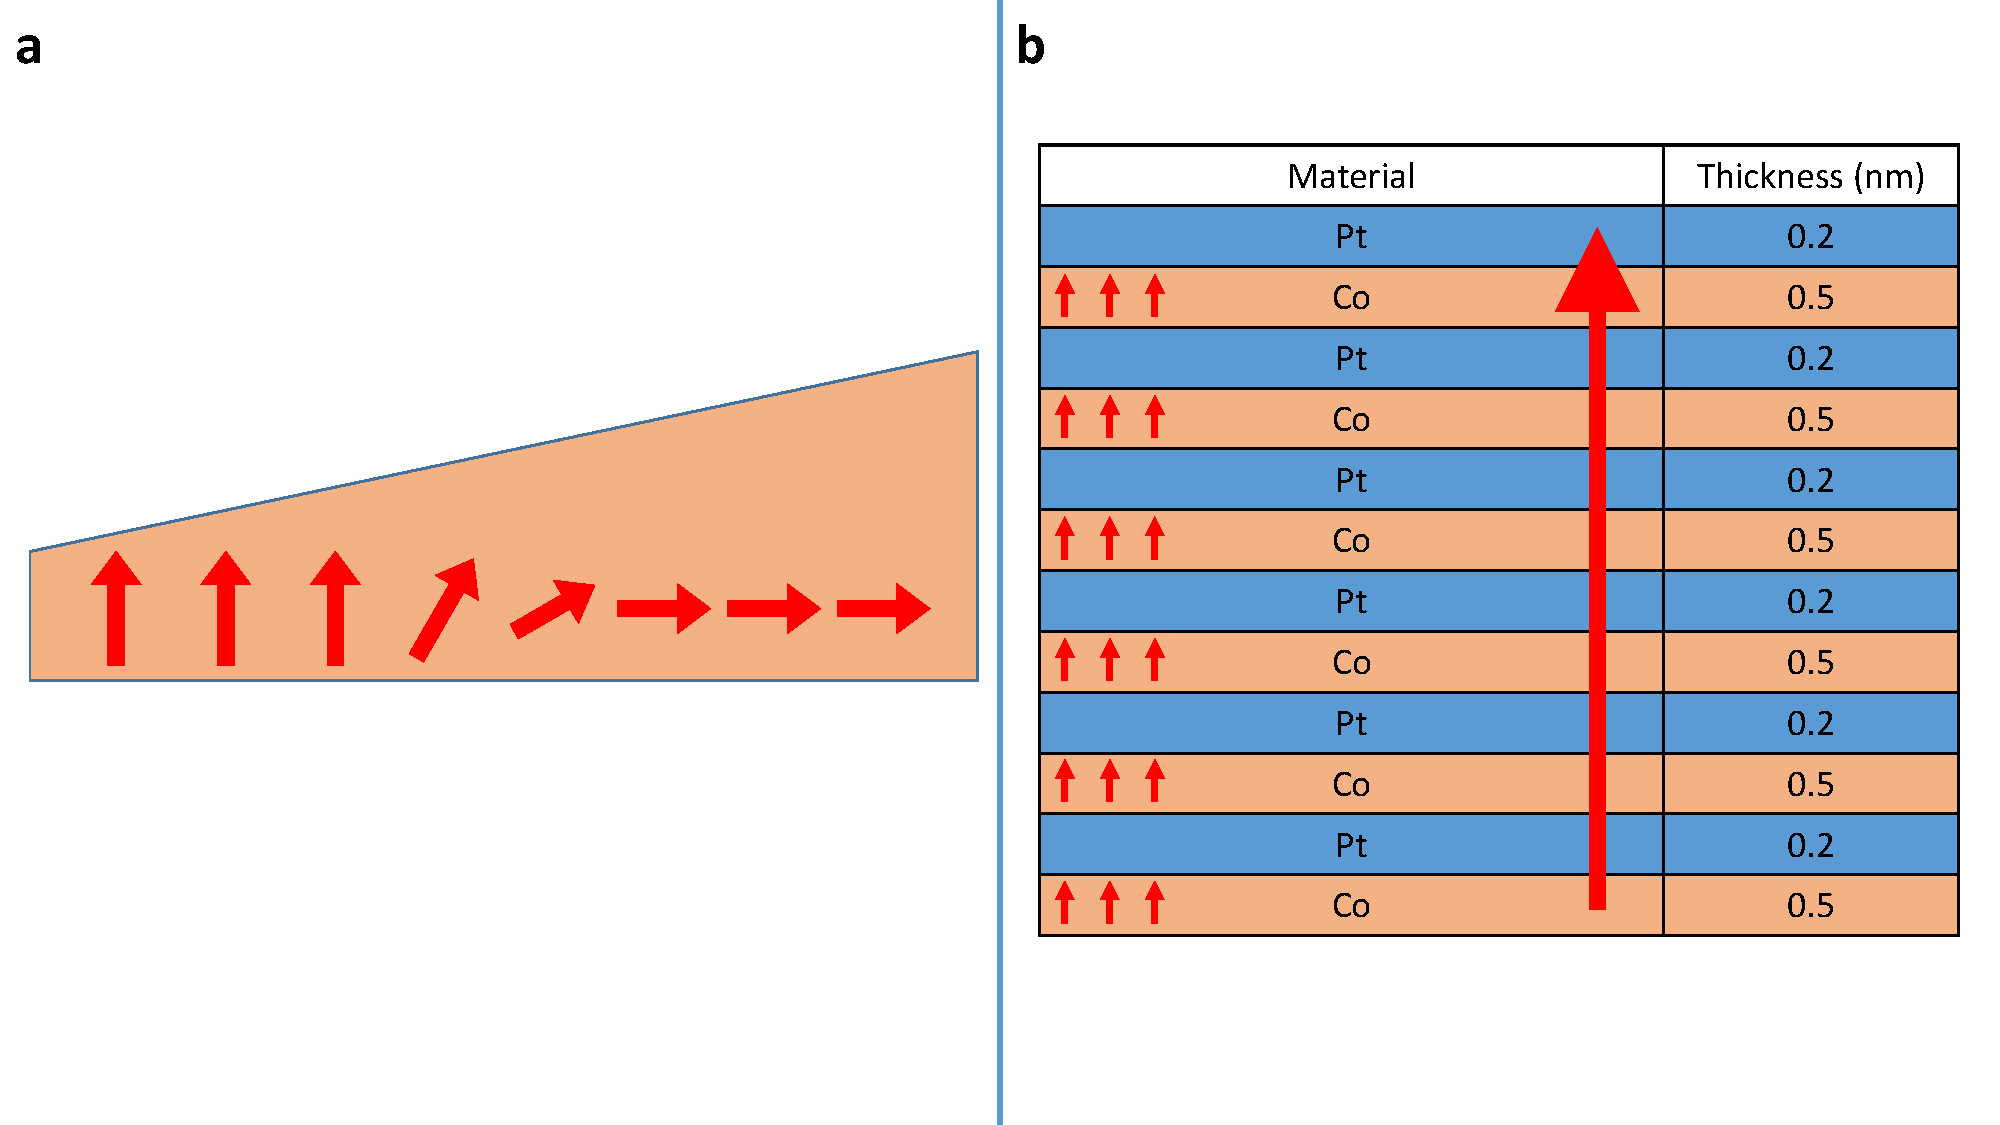
\includegraphics[width=0.75\paperwidth, page=1]{img/03/P_anisotropy_all.pdf}
        \caption{a) As the thickness of FM layer (light red) decreases, the magnetization (red arrows) tends to prefer perpendicular orientation (PMA), rather than IP anisotropy observed in thicker layers. b) Exemplary [$Co/Pt$] multilayer stack that exhibits PMA.}
        \label{PrinciplesPerpendicular}
    \end{figure}

\section{Storage element overview} \label{sec:PrinciplesStorageElement}

    Using all principles presented in Sections \ref{sec:PrinciplesMTJ} through \ref{sec:PrinciplesAdditionalPerpendicular}, a functional storage element can be built (Fig. \ref{PrinciplesMTJsum}). The prototype MRAM storage element, manufactured on $Si$ substrate consists of:
    
    %noitemsep, 
    \begin{itemize}[label=\textbullet]
    	\item metallic bottom electrode
    	\item synthetic anti-ferromagnet structure (SAF), that defines reference layer (RL) magnetisation
    	\item thin tunnel barrier
    	\item free layer (FL), that is used as a storage layer
    	\item metallic top electrode
    \end{itemize}
    
    \begin{figure}[H]
        \centering
        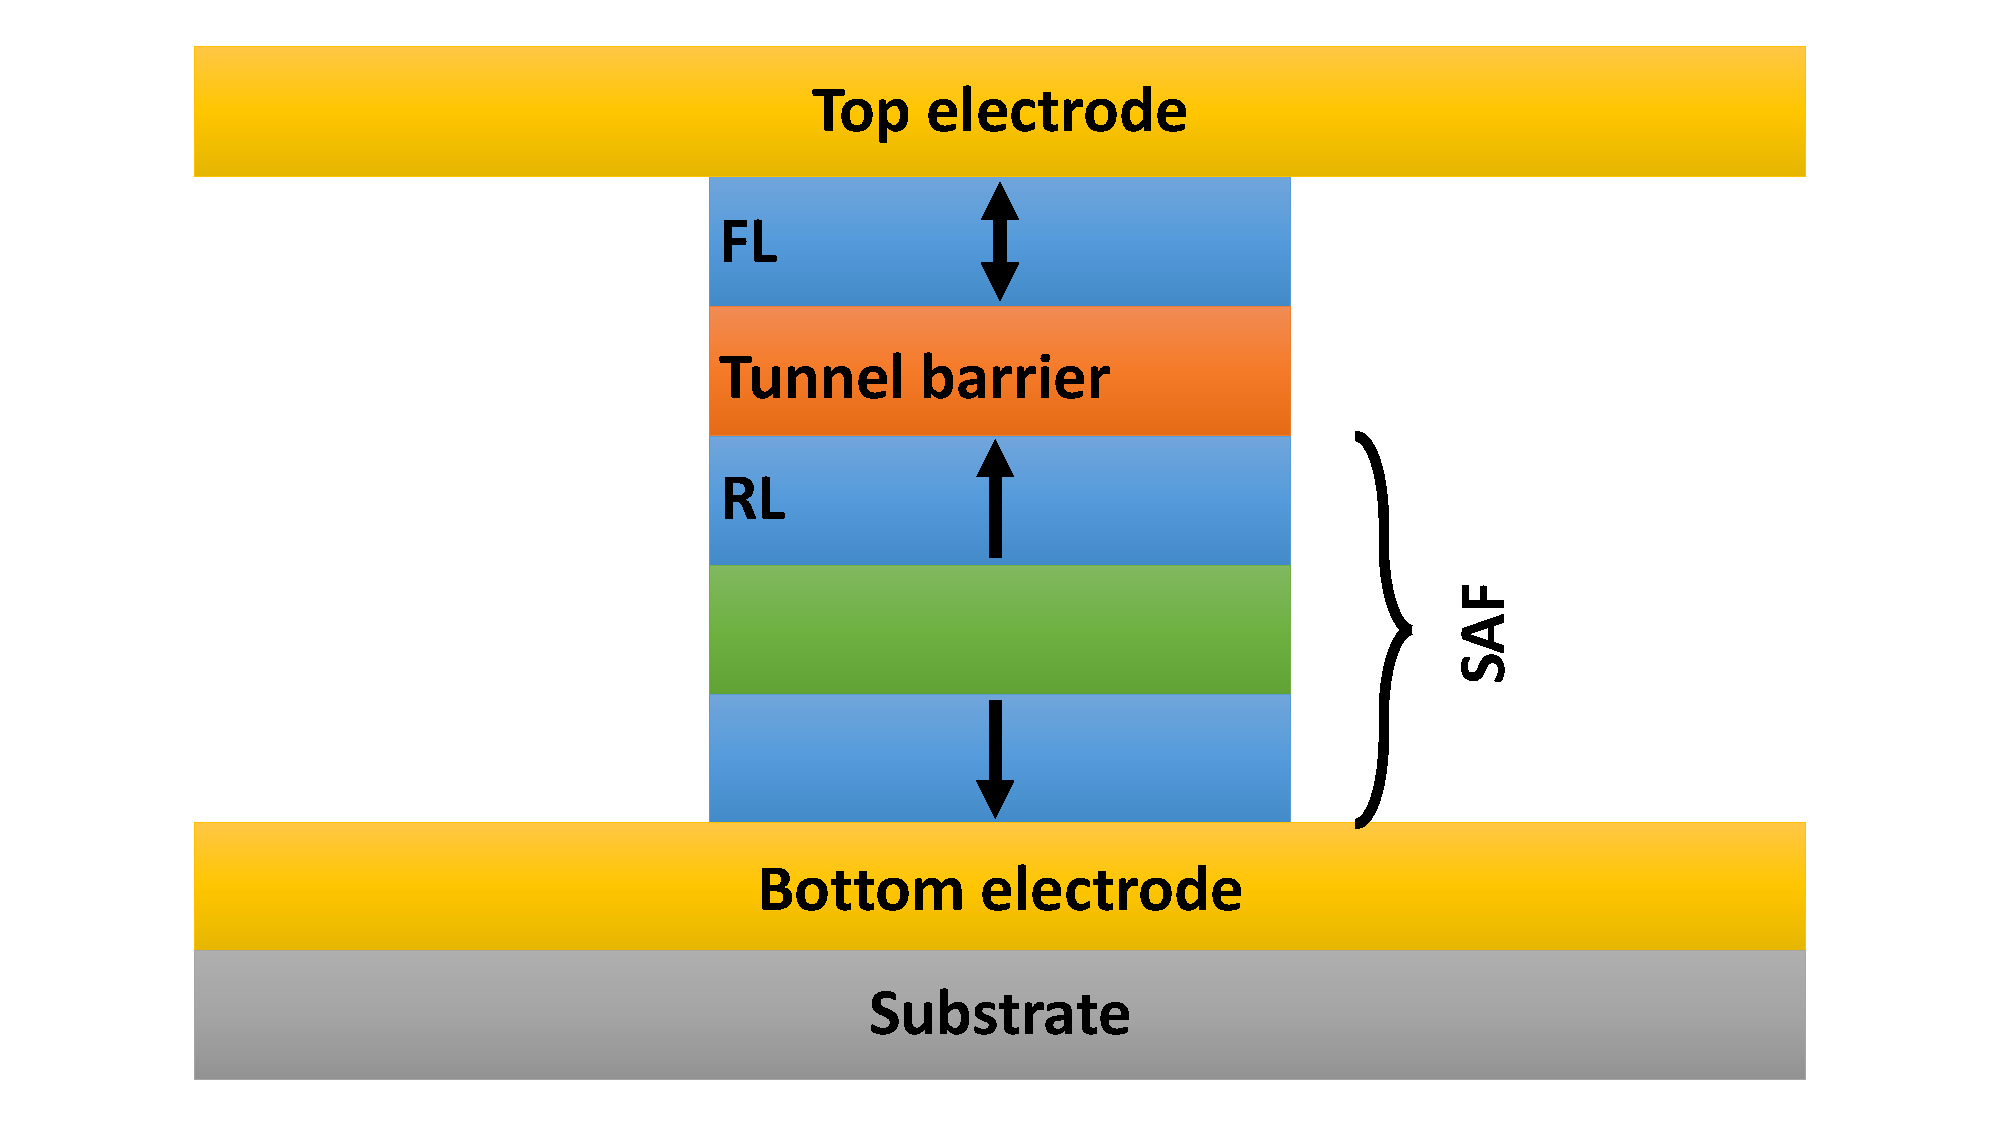
\includegraphics[width=0.75\paperwidth, page=1]{img/03/MTJ_summary.pdf}
        \caption{Schematic overview of functional MRAM storage element (MTJ).}
        \label{PrinciplesMTJsum}
    \end{figure}    
    
    The presented behaviour explains the usage of the MTJ as a storage element in MRAM memories - applying voltages lower than required to induce CIMS allows to measure the resistance (read the value), while applying sufficiently higher voltages results in writing the value.
    
\section{Theoretical analysis of the serial connection of storage elements} \label{sec:PrinciplesSerial}

	One of the possible arrangements of MTJs in a storage cell is a serial connection, where bottom contact of the first element is connected to the top contact of the next element, as shown in Fig. \ref{PrinciplesSeriesCon}.
	
	\begin{figure}[H]
        \centering
        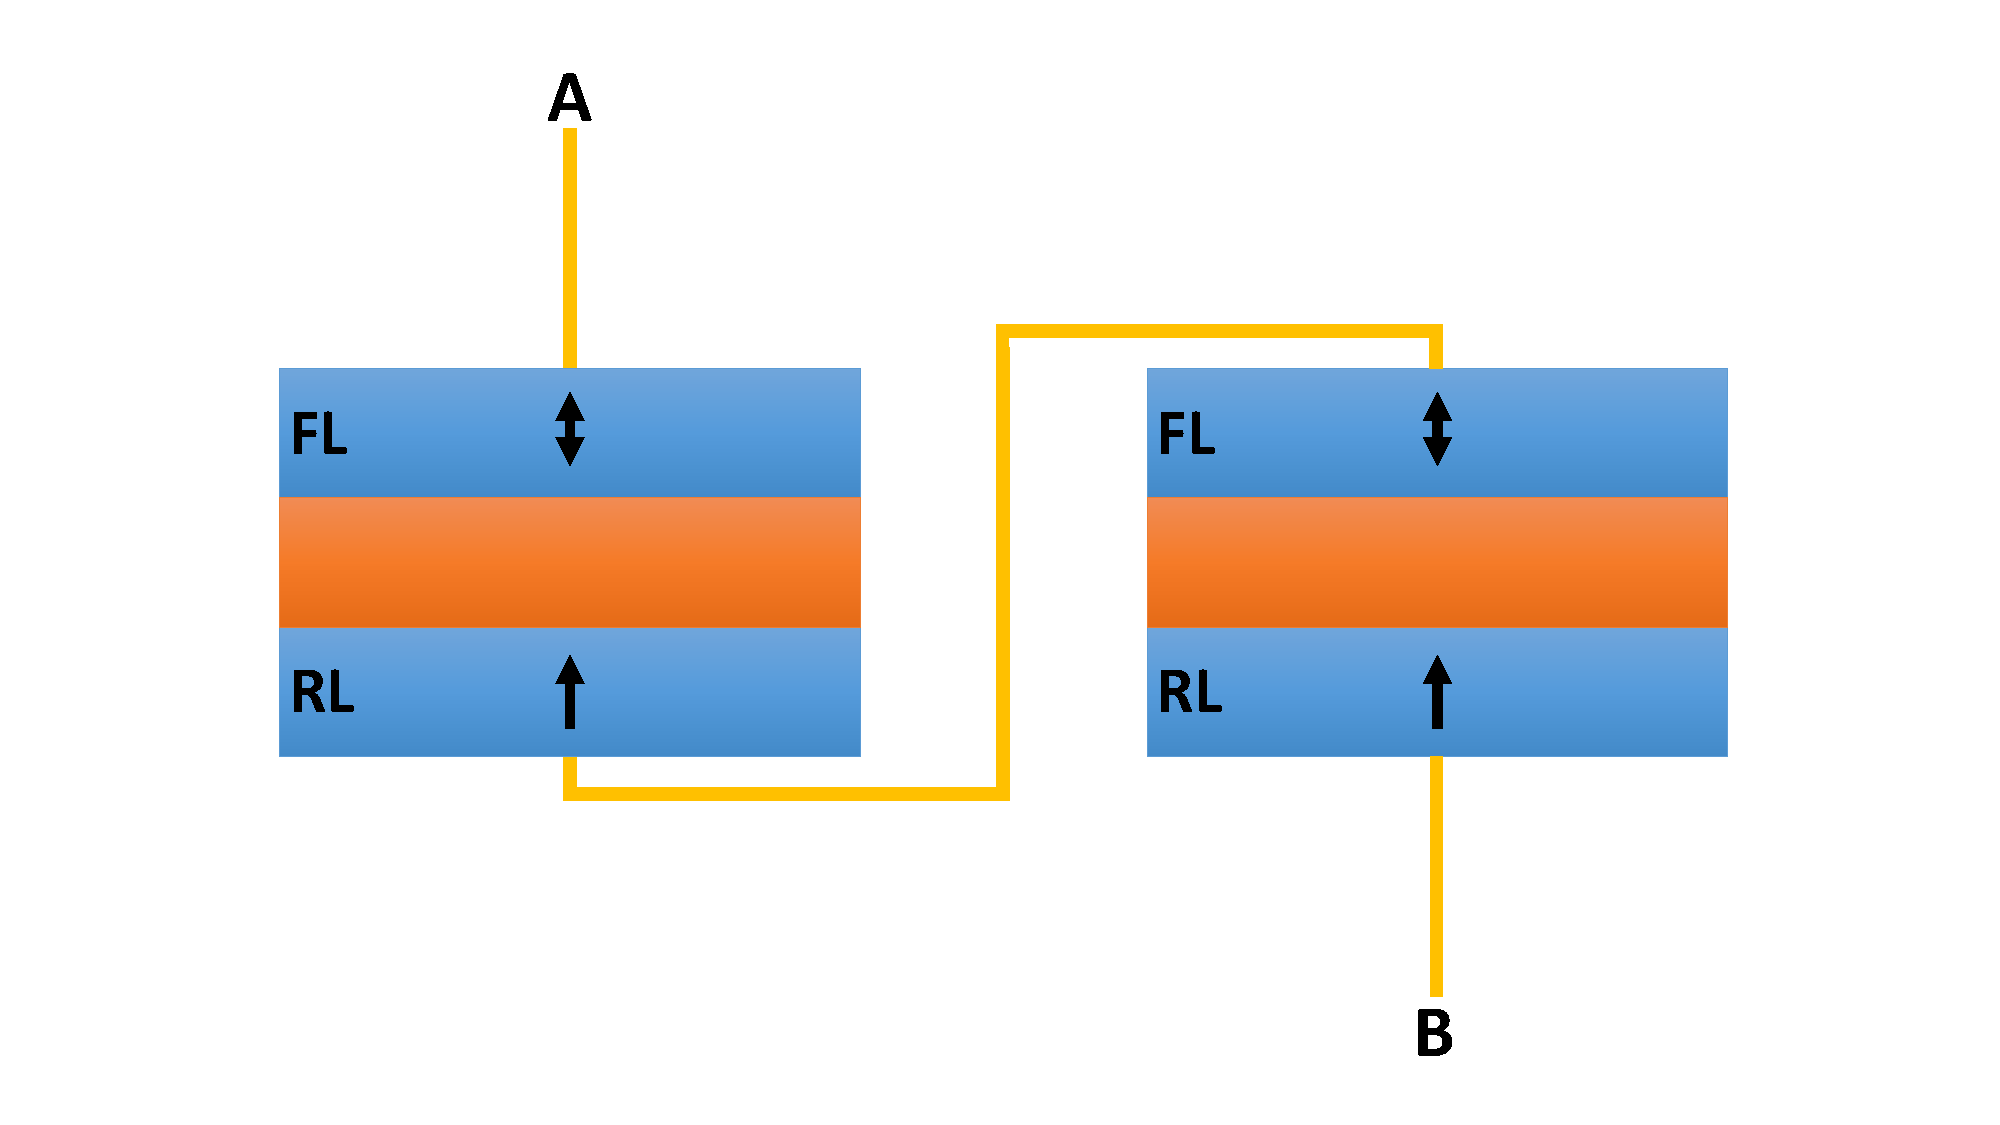
\includegraphics[width=0.75\paperwidth, page=1]{img/03/Series.pdf}
        \caption{Schematic of serial connection of two MTJs. A and B denote two ports of the storage cell.}
        \label{PrinciplesSeriesCon}
    \end{figure}
    
    The behaviour of the presented arrangement of storage elements can be predicted by analysing characteristics of a single MTJ (Fig. \ref{PrinciplesMTJcims}). If both junctions are in P state lowest resistance is observed. When negative voltage is applied, the current increases, until it reaches critical value inducing CIMS. The CIMS occurs only in one element, as it is a stochastic process. As one of the elements switches to AP state, with constant voltage applied, the current decreases. This prevents the other element from switching, as the current drops below the critical value. By further increasing the voltage, the critical current is reached again, and the second MTJ switches to AP state.
    
    By changing polarisation of the current, switching to the P state can be achieved. In the case, as soon as the critical current is reached, one of the elements switches to P state. With constant voltage applied, the current rises even higher above the critical value, causing the other element to switch to P state. 
    
    The complete characteristics, presenting this behaviour are presented in Fig. \ref{PrinciplesSeriesCIMS}. The above mechanism is believed to work also for more than two elements, as similar reasoning can be carried out. For the series connection utilizing the presented mechanism, $N+1$ stable resistance states would be observed for $N$ elements connected. This is because there is no possibility to individually determine the states of all incorporated storage elements - only number of elements in P and AP state may be determined, based on the resistance measurement.
    
    The storage cell capable of storing two bits of data would therefore consist of three serially connected storage elements. The predicted characteristics of such storage cell are presented in Fig. \ref{PrinciplesCIMS3bit}. Voltages for writing different states, as well as reading the cell can be defined. It is important to notice, that there is no possibility to reduce the resistance gradually.
    
    \begin{figure}[H]
        \centering
        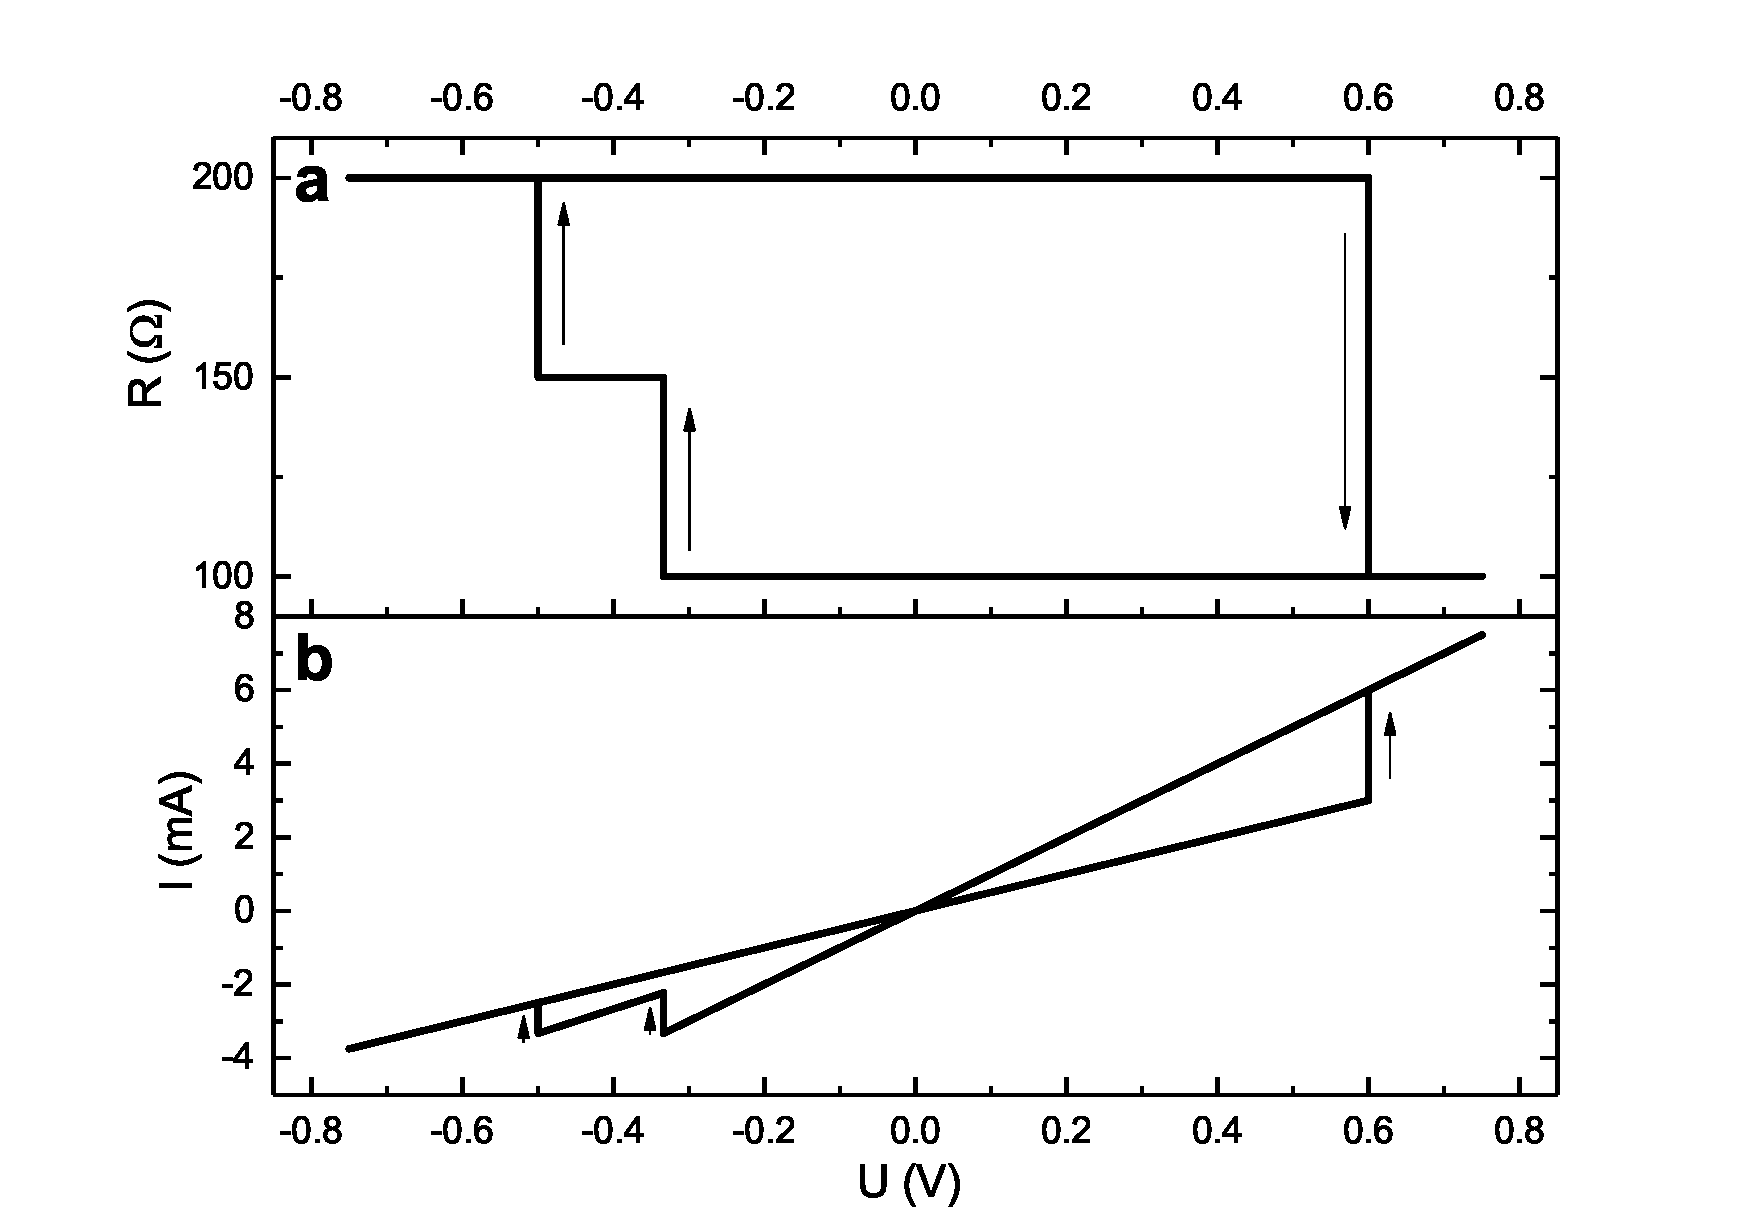
\includegraphics[width=0.6\paperwidth]{img/03/Series_characteristics.eps}
        \caption{Theoretically predicted a) resistance and b) current versus voltage applied to a storage cell constructed by use of two serially connected MTJs.}
        \label{PrinciplesSeriesCIMS}
    \end{figure}
    
    \begin{figure}[H]
        \centering
        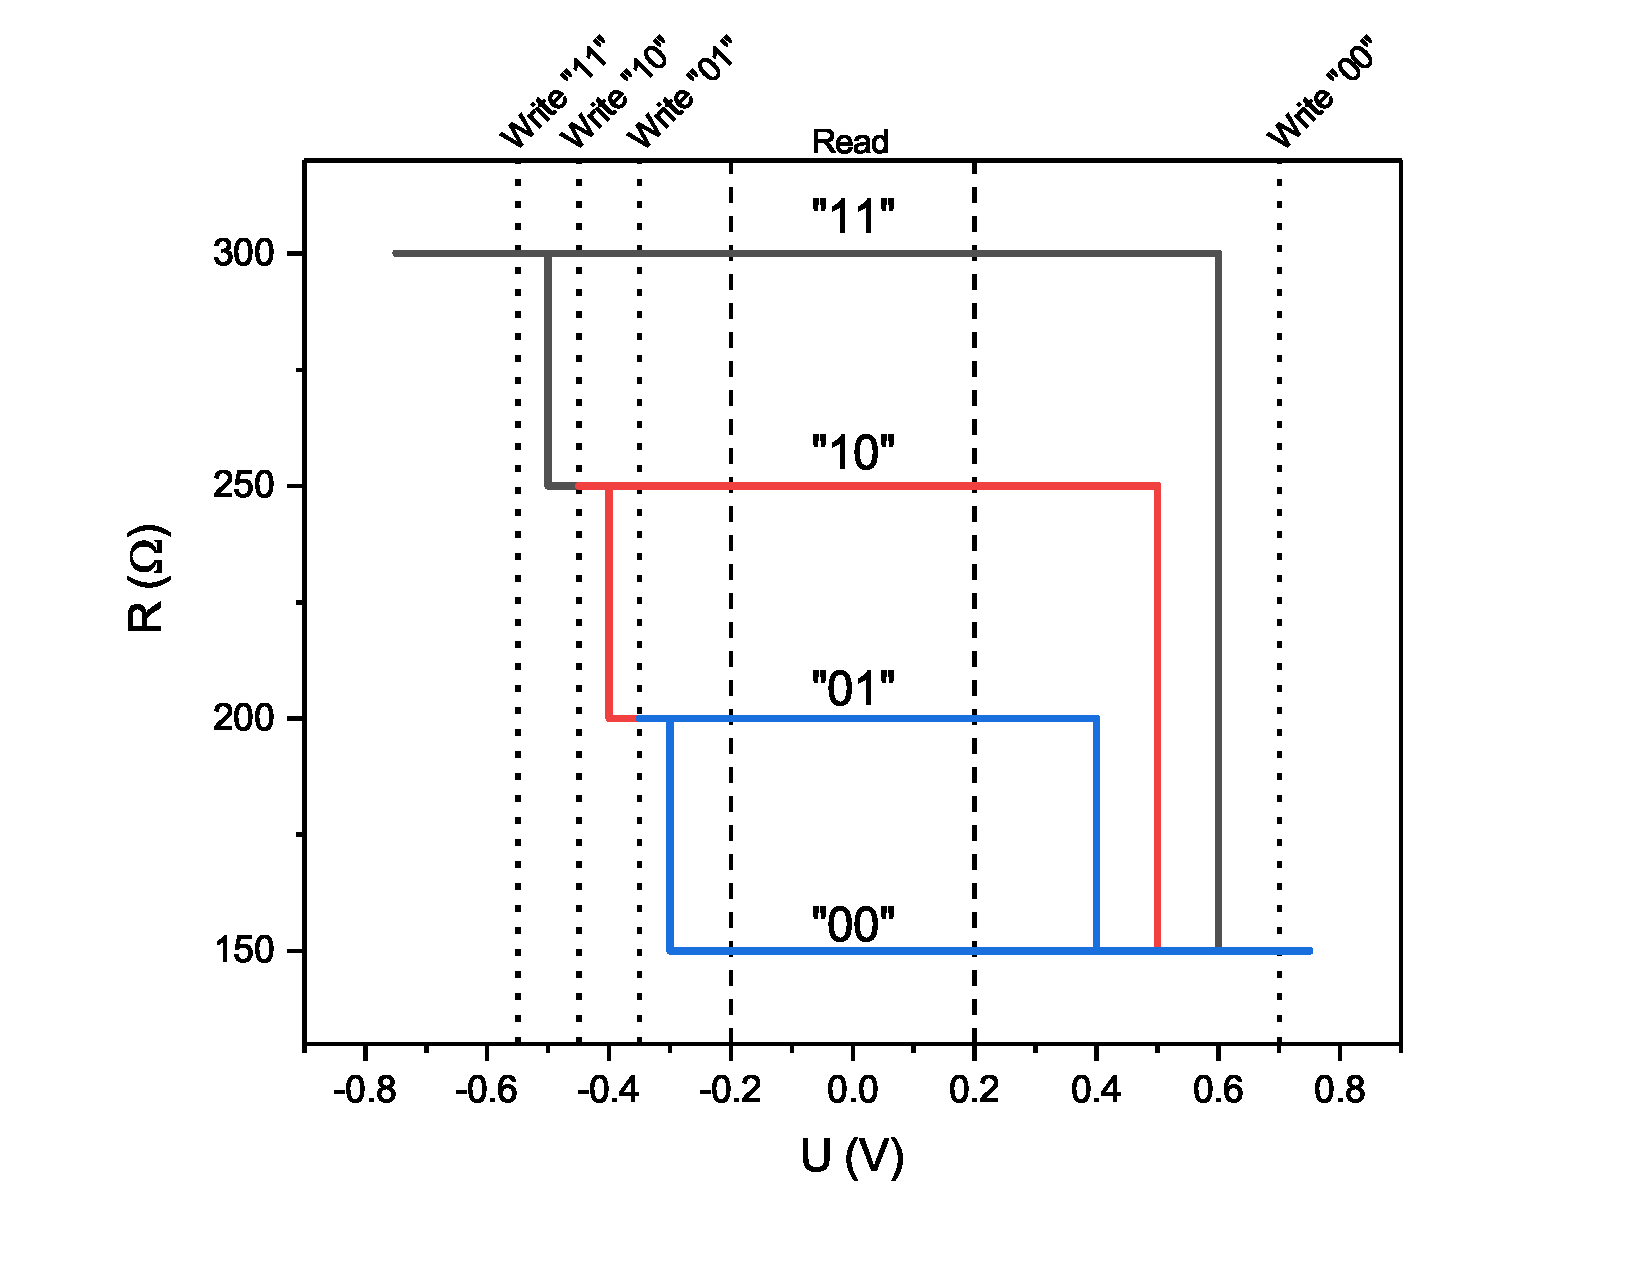
\includegraphics[width=0.6\paperwidth]{img/03/Series_3bit.eps}
        \caption{Theoretically predicted resistance versus voltage applied to a storage cell constructed by use of three serially connected MTJs. Possible mapping between resistance and binary value as well as proposed voltages to write and read the cell are marked on the plot. Different colours represent behaviour after writing different values.}
        \label{PrinciplesCIMS3bit}
    \end{figure}
    
\section{Theoretical analysis of behaviour of the parallel connection of storage elements} \label{sec:PrinciplesParallel}
    
    Driving storage elements connected in parallel with constant voltage would cause all of them to switch in nearly the same moment, therefore no interesting behaviour would be observed. The parallel connection may exhibit interesting behaviour when driven with constant current, but in this case the highest current would always flow through the element with the lowest resistance (P state). Therefore, switching other storage elements would require to pass higher current through the element in P state, with an increasing possibility to permanently damage it. Also taking into consideration a need to incorporate a precise variable current source into the memory design, this arrangement will not be the subject of the experimental part of this work. However, parallel connections may be in the area of interest when considering spin torque oscillators or microwave spin detectors.
    
\chapter{Fabrication techniques}
\label{sec:Fabrication}

This chapter presents MTJ stacks used for the experiment and describes the complete fabrication process of the sample.

\section{MTJ stack deposition for static devices} \label{sec:FabricationStackStatic}

    Based on previous experiments \cite{skowronski2017understanding}, an MTJ layer structure with PMA was proposed and deposited by Singulus AG using TIMARIS sputtering system in $Ar$ atmosphere on an oxidised $Si$ substrate. The substrate was etched before the deposition using ion etching, in order to clean the surface. The layer structure is presented in Tab. \ref{tab:FabricationLayerStructure}. 
    
    Layers 37-35 form a buffer, which reduces the surface roughness and induces proper crystal growth of other layers \cite{banasik2015magnetic}. Layers 34-8 form a SAF, with a reference layer (10-8) on the top. $Co/Pt$ layers 34-21 form a superlattice with strong PMA (Sec. \ref{sec:PrinciplesAdditionalPerpendicular}) which is coupled antiferromagnetically to another $Co/Pt$ superlattice (19-12) through a \SI{0.8}{\nano\meter} $Ru$ spacer (20). A composite reference layer (10-8) is also coupled through thin W layer (which, in addition, serves as a texture break), completing the SAF. A \SI{0.89}{\nano\meter} thick $MgO$ is used as a tunnel barrier (7), which results in the resistance area (RA) product of around \SI{20}{\ohm\times\micro\metre\squared}. Above, a composite free layer is placed (6-4). An important part of the top capping (3-1) is another $MgO$ layer (3), which increases PMA of the free layer.
    
    After the deposition process the sample was annealed at \SI{380}{\celsius} for \SI{60}{\minute}. The process allowed to relax interface stresses of the layers.
    
    \begin{table}[H]
    	\caption{Layer structure of the sample used for experiment, from top to bottom.}
    	\label{tab:FabricationLayerStructure}

    	\begin{center}
    	  \begin{tabular}{r r l l@{\hspace{20pt}} l}
    	    No. & Material & \multicolumn{3}{l}{Thickness (\SI{}{\nano\meter})} \\ \hline
    	    1 & $Ru$ 	& \cellcolor{capping}5.00 & \rdelim\}{3}{3mm}[Top capping] \\
    	    2 & $Ta$ 	& \cellcolor{capping}3.00 \\
    	    3 & $MgO$ 	& \cellcolor{capping}1.00 \\ \hline
    	    4 & $CoFeB$ & \cellcolor{ferromagnetic}0.50 & \rdelim\}{3}{3mm}[Free layer] \\
    	    5 & $W$ 	& \cellcolor{ferromagnetic}0.30 \\
    	    6 & $CoFeB$ & \cellcolor{ferromagnetic}1.30 \\ \hline
    	    7 & $MgO$	& \cellcolor{barrier}0.89 & Tunnel barrier \\ \hline
    	    8 & $CoFeB$ & \cellcolor{ferromagnetic}1.00 & \rdelim\}{3}{3mm}[Reference layer] & \rdelim\}{13}{3mm}[SAF] \\
    	    9 & $W$		& \cellcolor{ferromagnetic}0.25 \\
    	    10& $Co$	& \cellcolor{ferromagnetic}0.90 \\
    	    11& $Ta$	& \cellcolor{ferromagnetic}0.15 \\
    	    12& $Pt$	& \cellcolor{ferromagnetic}0.20 \\
    	   \ldelim\{{2}{3mm}[13\textasciitilde 18]& $Co$ & \cellcolor{ferromagnetic}0.50 & \rdelim\}{2}{3mm}[$\times 3$] \\
    	    &   $Pt$	& \cellcolor{ferromagnetic}0.20 \\
    	    19& $Co$	& \cellcolor{ferromagnetic}0.60 \\
    	    20& $Ru$	& \cellcolor{ferromagnetic}0.80 \\
    	    21& $Co$	& \cellcolor{ferromagnetic}0.60 \\
    	    \ldelim\{{2}{3mm}[22\textasciitilde 33] & $Pt$ & \cellcolor{ferromagnetic}0.20 & \rdelim\}{2}{3mm}[$\times 6$] \\
    	    &   $Co$	& \cellcolor{ferromagnetic}0.50 \\
    	    34& $Pt$	& \cellcolor{ferromagnetic}1.50 \\ \hline
    	    35& $Ta$	& \cellcolor{bottom}0.70 & \rdelim\}{3}{3mm}[Bottom buffer] \\
    	    36& $Ru$	& \cellcolor{bottom}7.00 \\
    	    37& $Ta$	& \cellcolor{bottom}2.00 \\ \hline
    	    & $SiO_2$ & \cellcolor{substrate} & \rdelim\}{2}{3mm}[Oxidised substrate]\\
    	    & $Si$ & \cellcolor{substrate} \\
    	  \end{tabular}
    	\end{center}
    \end{table}

\section{MTJ stack deposition for dynamic devices} \label{sec:FabricationStackDynamic}
\lipsum

\chapter{Electrical measurements}
\label{sec:Experiment}

    This chapter describes the experimental setup, and presents the results of the measurements taken.
    
\section{Static characterisation} \label{sec:ExperimentStatic}
\lipsum
   
\section{Dynamic characterisation} \label{sec:ExperimentDynamic}
\lipsum
\chapter{Application areas}
\label{sec:Fabrication}

This chapter presents application areas, where presented and characterised in this thesis devices may be useful.

\section{Multi-bit MRAM storage cells} \label{sec:MRAM}
\lipsum

\section{Neuromorphic computing} \label{sec:Neuromorphic}
\lipsum

\section{Precise oscillators} \label{sec:Oscillator}
\lipsum
\chapter{Future work}
\label{sec:FutureWork}
\lipsum

\chapter{Summary}
\label{sec:Summary}
\lipsum
    

\chapter{Acknowledgements}

	This work is supported by the Polish Ministry of Science and Higher Education \textbf{Diamond Grant No. 0048/DIA/2017/46} and the Polish National Center for Research and Development grant No. \textbf{LIDER/467/L-6/14/NCBR/2015}.
	
    \vspace{2cm}
    
    I would like to express my profound gratitude to \textbf{my parents}, for their support and invaluable help at every moment of my life.

    I would like to thank my supervisor, \textbf{PhD Witold Skowroński}, for his help in preparing the work and carrying out the experiments.

	I am very grateful to \textbf{Professor Tomasz Stobiecki}, for giving me an opportunity to explore the world of science.

    I would like to thank \textbf{PhD Sławomir Ziętek}, for his help in carrying out the experiments.
    
    I am grateful to \textbf{Academic Center of Materials and Nanotechnology (ACMiN AGH)} and \textbf{Professor Marek Przybylski} for an opportunity to perform nanostructurization of the sample. I would also like to thank \textbf{Singulus AG} and \textbf{PhD Jerzy Wrona} for providing the sample with MTJ stack deposited.





%\appendix
\printbibliography

\end{document}
